\documentclass[conference]{IEEEtran}
\IEEEoverridecommandlockouts
% The preceding line is only needed to identify funding in the first footnote. If that is unneeded, please comment it out.
\usepackage{cite}
\usepackage{amsmath,amssymb,amsfonts}
\usepackage{algorithmic}
\usepackage{graphicx}
\usepackage{textcomp}
\usepackage{xcolor}
\usepackage{hyperref}
\usepackage{caption}
\usepackage{subcaption}
\usepackage{booktabs}


\def\BibTeX{{\rm B\kern-.05em{\sc i\kern-.025em b}\kern-.08em
    T\kern-.1667em\lower.7ex\hbox{E}\kern-.125emX}}
\begin{document}

\title{Guidance, Navigation, and Control of an Autonomous X-wing Fighter}

\author{\IEEEauthorblockN{Arthicha Srisuchinnawong}
\IEEEauthorblockA{
\textit{University of Southern Denmark, Odense, Denmark} \\
arsri21@student.sdu.dk}
}

\maketitle

\begin{abstract}
	This project aims to verify if existing guidance, navigation, and control techniques can achieved a comparable simulation result to the science friction spaceship, star wars' x-wing fighter, introduced nearly 50 years ago. With lookahead-based line-of-sight guidance system, Kalman state estimation, along with proportion-derivative control, the simulated x-wing fighter can navigate and perform a surveillance mission; however, the control parameters are sensitive and have to be selected carefully.
\end{abstract}

\begin{IEEEkeywords}
Guidance, Navigation, Control, Modeling, Simulation
\end{IEEEkeywords}

\section{Introduction}
Star wars is a multimedia science fiction franchise firstly introduced in 1977 \cite{starwars}. It involves a famous spaceship called "X-wing Fighter" as illustrated in Fig.~\ref{fig:overview}(a). The spaceship consists of four winds forming X-shape, and it is able to take off vertically and battle in space. 

At that time, the real-world technology was still far from what mentioned in the science friction. As the time pass, people have developed new advanced technologies and advanced technique for controlling spacecrafts. Nowadays, we have seen many kind of robots, such as, autonomous mobile robot \cite{mir} that navigate throughout unseen space and autonomous quadrature drone \cite{mpc_drone,scimet_paper} with robust control strategy and advanced localization technique. These are the evidences that we are stepping closer to sci-fi movies. 

Therefore, this project aims to study and verify whether existing guidance, navigation, and control approaches is able to achieved what people in 1977 had imagined or not, and to which degree we are able to achieved it nowadays. In this works, the X-wing fighter is modeled as described in section~\ref{sec:model}. The guidance system is then discussed in section~\ref{sec:guidance}, following by the control described in  section~\ref{sec:control} and the state estimation described in  section~\ref{sec:statestimation}. The aforementioned process is then section~\ref{sec:experiment}, before the result is discussed and concluded in section~\ref{sec:conclusion}.

\section{Autonomous X-wing Fighter}

The control system of the autonomous x-wing fighter is shown in Fig.~\ref{fig:overview}. Overall, after a state estimator (Fig.~\ref{fig:overview}(h–i)) estimates the x-wing fighter's pose, a guidance system (Fig.~\ref{fig:overview}(g)) produces desired velocities, telling the direction toward waypoints. A controller (Fig.~\ref{fig:overview}(e–f)) then stabilizes and produces actuator commands sending to the x-wing fighter model (Fig.~\ref{fig:overview}(b–d)) to stabilize and move the fighter accordingly. Finally, the x-wing fighter is visualized in a simulation (Fig.~\ref{fig:overview}(a)). The github repository of this project is available at \href{https://github.com/Arthicha/Guidance-Navigation-and-Control-of-an-Autonomous-X-wing-Fighter}{\url{https://github.com/Arthicha/Guidance-Navigation-and-Control-of-an-Autonomous-X-wing-Fighter}}

\begin{figure*}[!htbp]
	\centering
	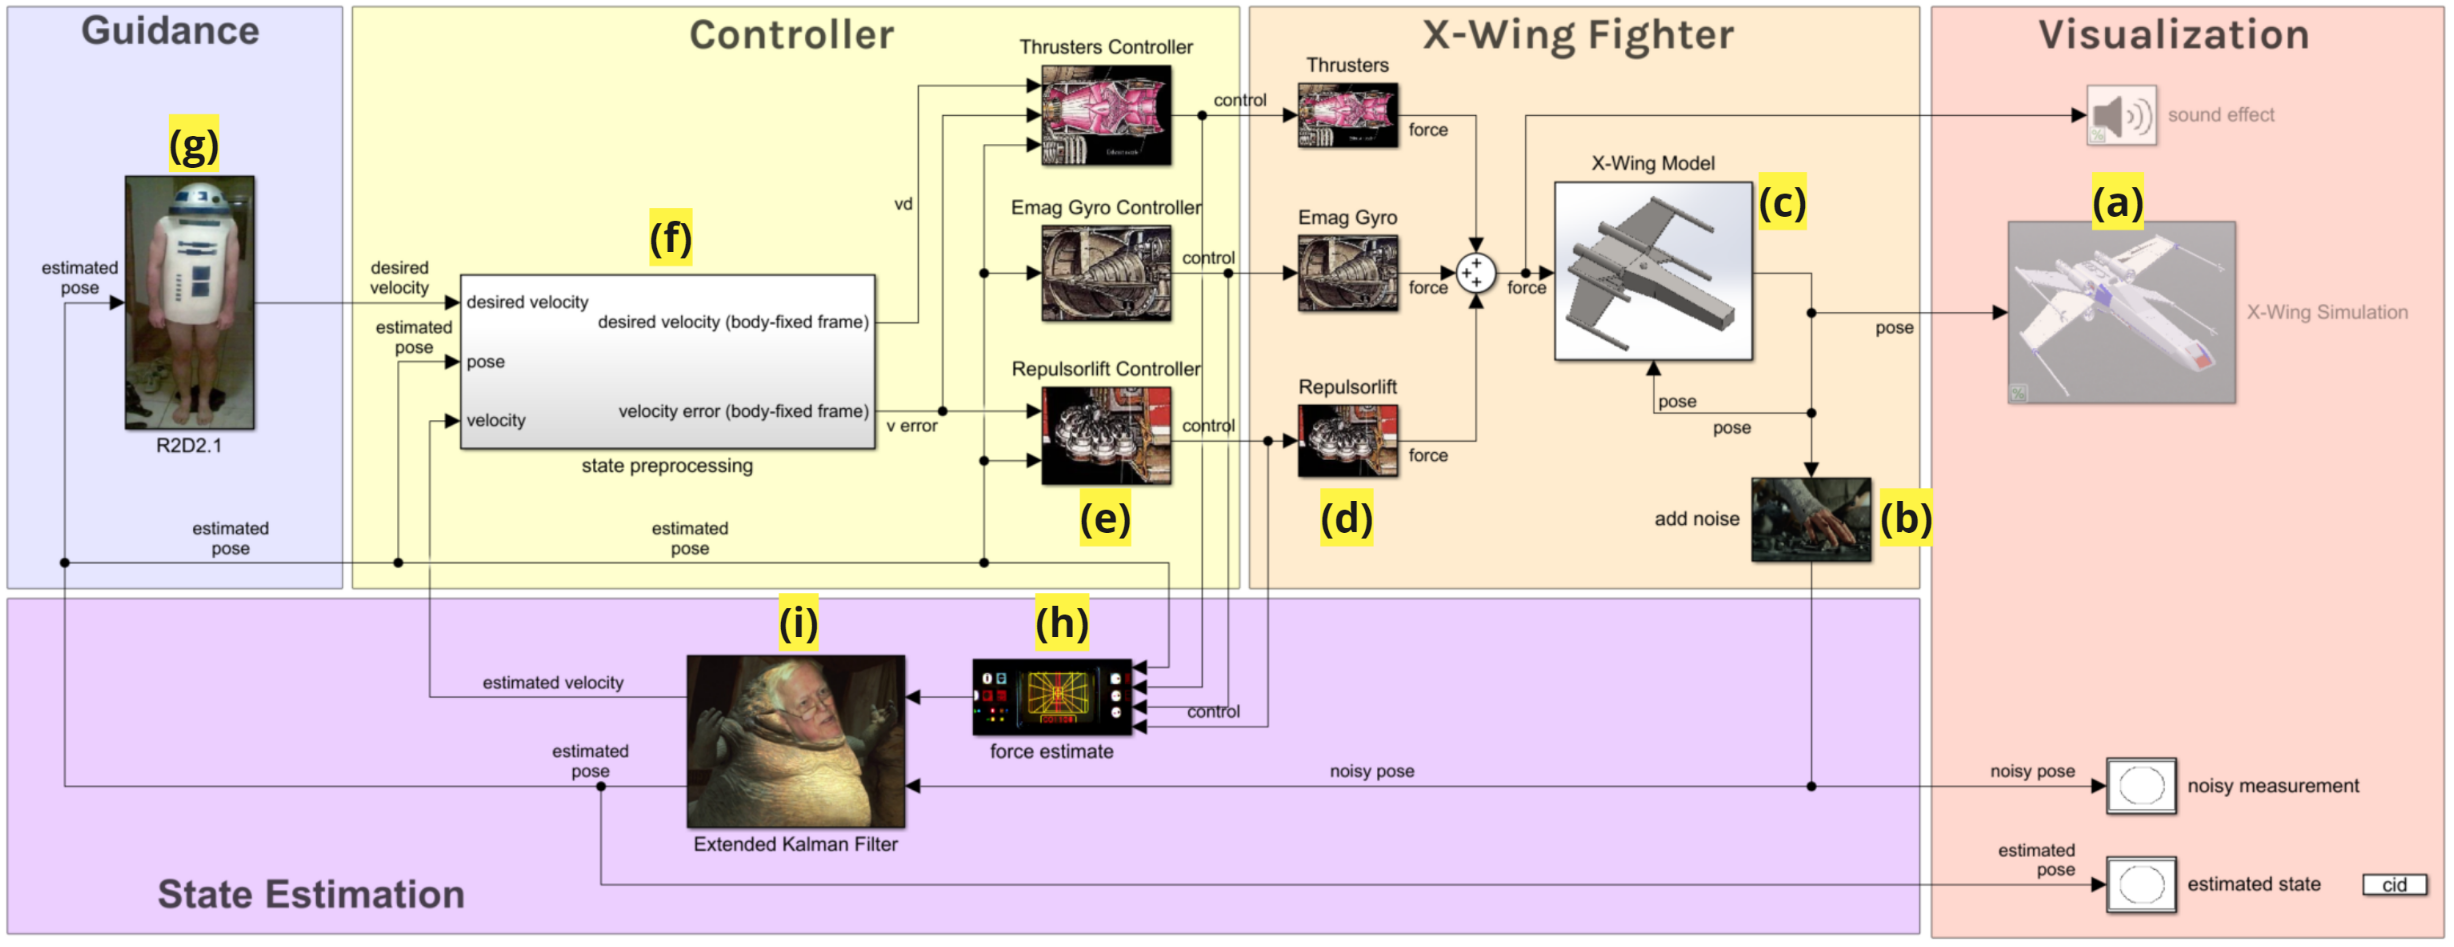
\includegraphics[width=0.85\linewidth]{figures/overview}
	\caption{Control system of the autonomous x-wing fighter, consisting of five key components: (a) simulation, (b–d) x-wing fighter model, (e–f) controller, (g) guidance system, and (h–i) state estimator.}
	\label{fig:overview}
\end{figure*}




\subsection{Modeling and Simulation}
\label{sec:model}
To simulate the behavior of the x-wing fighter, we assume three actuators: differential thrusters, electromagnetic gyroscopic stabilizer \footnote{A gyroscopic stabilizer, also known as a gyro-stabilizer, is a system of gyroscopes, hydraulics and high-speed processors \cite{gyros}.} \cite{gyros}, and repulsorlift \footnote{Repulsorlift is a technology that allowed a craft to hover or even fly over a planet's surface by pushing against its gravity, producing thrust \cite{repulsorlift}.} \cite{repulsorlift}. Force and moment are the combinations of four terms: force and moment from the differential thrusters, from gyro-stabilizer, repulsorlift, and gravitational force. For simplicity, the central of gravity is assumed to be in the center of the spaceship, and all forces and moments are assumed acting at that location. The total force and moment are computed from equation~\ref{eq:sumforce}–\ref{eq:thrusterforce}.
\begin{equation}
\begin{bmatrix} F^b \\ M^b \end{bmatrix} = \kappa
\begin{bmatrix} u_{t1} \\ u_{t2} \\ u_{t3} \\ u_{t4} \end{bmatrix}
+ k_4 u_{gy} + k_5 u_{re} + \begin{bmatrix} F_g^b \\ 0 \\ 0 \\ 0 \end{bmatrix},
\label{eq:sumforce}
\end{equation}
\begin{equation}
\kappa = \begin{bmatrix} k_1 & k_1 & k_1 & k_1\\
0 & 0 & 0 & 0 \\
0 & 0 & 0 & 0 \\
0 & 0 & 0 & 0 \\
-k_2 & -k_2 & k_2 & k_2 \\
k_3 & -k_3 & k_3 & -k_3 
\end{bmatrix},
\label{eq:thrusterforce}
\end{equation}
where $F^b$ and $M^b$ denotes the force and moment applied at the center of mass of the spaceship and with respect to in body-fixed frame; $u_{ti}$, $u_{gy}$, and $u_{re}$ denotes the control input to the $i^th$ thruster, gyro-stabilizer, and repulsorlift, respectively; $F^b_g$ denotes the gravitational force expressed in the body-fixed frame, and $k_1$–$k_5$ denote the gain which are found to be $2.5\times10^3$, $6.8\times10^3$, $1.425\times10^4$, $1.0\times10^4$ and $1.0\times10^4$, respectively\footnote{All gains are computed from the kinematics of the x-wing fighter}. Note that, lifting force is excluded here due to the symmetric structure of the wings.

In this work, gravitational force is modeled as variable term with inverse relationship with the height, as shown in equation~\ref{eq:gravitationalforce}.
\begin{equation}
F_g^b = R^w(\Theta^w)^T \begin{bmatrix} 0 \\ 0 \\ \frac{GmM_e}{r^2} \end{bmatrix} ,
\label{eq:gravitationalforce}
\end{equation}
 where $R^w(\Theta^w)$ denotes the rotation matrix computed from spaceship orientation with respect to the world-fixed frame, $G$ denotes the gravitational constant which is $6.6726\times10^{-11}~ Nm^2/kg^2$, $M_e$ denotes the earth mass which is $5.98\times10^{24}~kg$, and $r$ denote the distance from the earth center.

The spaceship pose with respect to world-fixed frame is modeled according to equation~\ref{eq:dynamic} and \ref{eq:velocity_transform}. To simulate measurement noise, white noise with zero mean and $[5\:\text{m}, 5\:\text{m}, 5\:\text{m}, 0.1\:\text{rad}, 0.1\:\text{rad},0.1\:\text{rad}]^T$standard deviation is also added to the pose.
\begin{align}
\begin{bmatrix} \dot{v}^b \\ \dot{\omega}^b \end{bmatrix} = \begin{bmatrix}mI & \underline{0} \\ \underline{0} & I_c \end{bmatrix}
^{-1} \left( 
\begin{bmatrix} F^b - m \left[ \omega^b \right]_\times v^b \\ M^b + \left[ I_c \omega^b \right]_\times \omega^b \end{bmatrix}
 \right ),
\label{eq:dynamic}
\end{align}
\begin{equation}
\begin{bmatrix} \dot{p}^w \\ \dot{\Theta}^w \end{bmatrix} = \begin{bmatrix}R^w(\Theta^w) & \underline{0} \\ \underline{0} & T(\Theta^w) \end{bmatrix} 
\begin{bmatrix} v^b \\ \omega^b \end{bmatrix},
\label{eq:velocity_transform}
\end{equation}
where $v^b$ and $\omega^b$ denote the spaceship twist (i.e., linear and angular velocity) with respect to in the body-fixed frame, $p^w$ and $\Theta^w$ denote the spaceship pose (i.e., position and orientation) with respect to in the world-fixed frame, $m$ denotes the mass which is 10,000 kg \cite{xwing_wiki}, $\underline{0}$ and $I$ denote 3-by-3 zero matrix and 3-by-3 identity matrix, respectively , $I_c$ denote the inertia matrix calculated from CAD software, $[\square]_\times$ denote the skew symmetric matrix, and $T(\Theta^w)$ denotes the transformation matrix transforming the velocity from body-fixed frame to world-fixed frame (i.e., from $\omega^b$ to $\Theta^w$).  


The spaceship pose with respect to in world-fixed frame is then converted from flat earth coordinate system to latitude-longitude-altitude coordinate system using standard MATLAB simulink block \cite{fe2lla}. Finally it is sent to the FlightGear \cite{flightgear} simulation to visualize the behavior.

\subsection{Guidance}
\label{sec:guidance}
The guidance system divides into two parts: a waypoint generator and a lookahead-based guidance law. The objective of the waypoint generator is to the lookahead-based guidance of the local goals (i.e., waypoints), while the look ahead guidance guides the spaceship toward such goals (in this case, we use desired velocity as our guidance output).

\subsubsection{Waypoint Generator}
The waypoint generator encoded the spaceship's airspace defense mission, as shown in Table~\ref{tab:waypoint} and Fig.~\ref{fig:exp_Dgain}. 

\begin{table}[!h]
	\caption{Airspace defense mission and the corresponding waypoints}
	\centering
	
	\begin{tabular}{@{}cll@{}}
		\toprule
		\textbf{\rotatebox[origin=c]{0}{ {index}}}  & 
		\textbf{\rotatebox[origin=c]{0}{waypoint (km)}}& 
		\textbf{\rotatebox[origin=c]{0}{description}}
		\\ \toprule
		1 & (x,y,z) = (0,0,0) & start location\\ 
		2 & (x,y,z) = (0,0,1) & vertical take off\\ 
		3 & (x,y,z) = (10,0,5) & departure \\ 
		4 & (x,y,z) = (30,30,100) & climb\\ 
		5 & (x,y,z) = (10,20,5) & descent \\ 
		6 & (x,y,z) = (7,7,5) & initial approach\\ 
		7 & (x,y,z) = (4,4,3) & middle approach\\ 
		8 & (x,y,z) = (0,0,3) & final approach \\ 
		10 & (x,y,z) = (0,0,0) & vertical landing \\ 
		\bottomrule
	\end{tabular}
	\label{tab:waypoint}
\end{table}

The objective of the mission is to navigate between those waypoints in straight lines. To deal with noise and disturbance, the waypoint generator output new waypoints only if the spaceship reaches the acceptance sphere, i.e., equation~\ref{eq:acceptance_sphere} is satisfied.
\begin{equation}
	||p^w(t) - p_i^{w*} || \leq \epsilon_r,
	\label{eq:acceptance_sphere}
\end{equation}
where $p^w(t)$ denotes the position of the x-wing fighter with respect to world-fixed frame, $p_i^{w*}$ denotes the $i^th$ waypoint, $||\square||$ denotes the second norm, and $\epsilon_r$ denotes the radius of the acceptance sphere which is set to a relatively small value of 2 km to ensure following the desired path. 


\subsubsection{Lookahead-based Guidance Law}
To follow the path described previously, lookahead-based line-of-sight guidance law is implemented. This approach includes two objectives: guiding the spaceship (1) toward and (2) to follow the path segment, i.e., straight line segment connecting between the previous and next waypoints.

\begin{figure}[h]
		\centering
		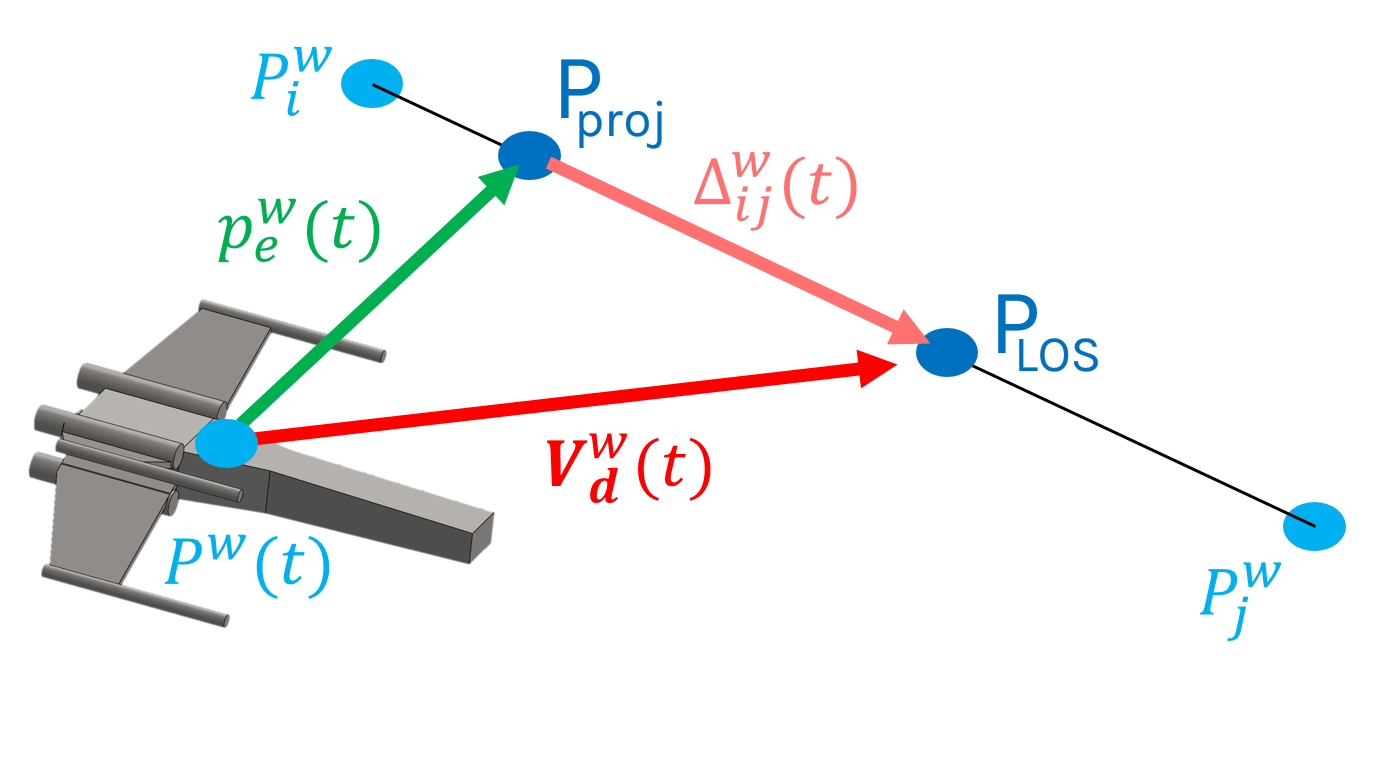
\includegraphics[width=0.7\linewidth]{figures/lookahead_normal.png}
	\caption{Graphic representation of line-of-sight position and the guidance/desired velocity.}
	\label{fig:lookahead}
\end{figure}

The line-of-sight position is computed according to:
\begin{equation}
p^w_{los}(t) = p^w_i + \Delta^w_{ij}(t) + p^w_e(t),
\label{eq:guidance_plos}
\end{equation}
where $p^w_{los}(t)$ denotes the light-of-sight position at time $t$, $p^w_i$ denotes the previous waypoint, $\Delta^w_{ij}(t)$ denotes the lookahead distance, and $p^w_e(t)$ denotes the distance toward the path segment. Note that, here, all value is computed with respect to the world-fixed frame.

The lookahead distance ($\Delta^w_{ij}(t)$) guides the spaceship to follow the path. It is computed from the unit vector of path segment according to:
\begin{equation}
\Delta^w_{ij}(t) = \frac{  \eta_\Delta  (p_j^i)}{||p_j^i||+\epsilon},
\label{eq:guidance_delta}
\end{equation}
where $p_j^i$ denotes the vector from the previous waypoint to the next waypoint, or rather, $p_j^i = p^w_j-p^w_i$, $\eta_\Delta$ denotes the gain defining the magnitude of lookahead distance (this parameter is analyzed in section~\ref{sec:exp_guidance}), and $\epsilon$ denotes an arbitrary small number which is $1.0\times10^{-6}$ in this case.

On the other hand, the distance toward the path ($p^w_e(t)$) guides the spaceship toward the path. It is computed from the projection point ($P_{proj}$) according to:
\begin{equation}
p^w_e(t) = \eta_e \left(    \frac{          (  p^i(t) \cdot p_j^i  )    p_j^i        }{||p_j^i||^2+\epsilon}         -p^i(t)  \right),
\label{eq:guidance_pe}
\end{equation}
where $p^i(t)$ denotes the vector from the previous waypoint to the spaceship's position, or rather, $p^i(t) = p^w(t)-p^w_i$, and $\eta_e$ denotes the gain defining the magnitude of lookahead distance (this parameter is analyzed in section~\ref{sec:exp_guidance}).

Lastly, the guidance/desired velocity ($v_d^w(t)$) is computed from:
\begin{equation}
v^w_d(t) = \left( p^w_{los}(t)-p^w(t) \right).
\label{eq:guidance_velocity}
\end{equation}




\subsection{Control}
\label{sec:control}
The control of the x-wing fighter consists of two parts: preprocessing (Fig~\ref{fig:overview}(f)) and three controllers (Fig~\ref{fig:overview}(e)). Firstly, the desired velocity from the guidance system (Fig~\ref{fig:overview}(g)) is combined with estimated pose and estimated velocity from the state estimation (Fig~\ref{fig:overview}(h–i)) to produce the reference signals for the controllers. The controllers include (1) a thruster controller producing the control command for differential thruster, (2) a gyroscopic stabilizer controller producing the control command for the gyro-stabilizer, and (3) a repulsorlift controller producing the control command for the repulsolift.


\subsubsection{Preprocessing}
In the preprocessing step, the desired velocity expressed in world-fixed frame is transform to the body-fixed frame ($v^b_d(t) $), which is then utilized for aligning the spaceship heading, according to section~\ref{sec:thruster_control}. The transformation is done according to:
\begin{equation}
v^b_d(t) = R^w(\Theta^w)^T v^w_d(t).
\label{eq:desired_velocity_body}
\end{equation}

Also, the velocity error in body-fixed frame ($\tilde{v}^b_d(t)$) are computed according to equation~\ref{eq:velocity_error_body}. The body-fixed frame error ($\tilde{v}^w_d(t) $) is employed to drive the x-wing fighter forward, upward, and to change the angle of attack. This will be described in more details in section~\ref{sec:thruster_control} and section~\ref{sec:repulsorlift_control}.
\begin{equation}
\tilde{v}^b_d(t) = v^b_d(t) - v^b(t).
\label{eq:velocity_error_body}
\end{equation}



\subsubsection{Thruster Controller}
\label{sec:thruster_control}
The thruster controller serves three main purposes: to directly control (1) the forward speed, (2) the heading direction, and to indirectly control (3) the attitude through the pitch angle. All aforementioned quantities are controlled using a standard PD control, according to equation~\ref{eq:PD_control}. 
\begin{equation}
u = K_p e(t) + K_d \frac{\Delta e(t)}{ \Delta t},
\label{eq:PD_control}
\end{equation}
where $u$ denotes the control input or the control command, $K_p$ and $K_d$ denote the proportion gain and derivative gain, respectively,  $e(t) $ denotes the error signal, and $\frac{\Delta e(t)}{ \Delta t}$ denotes the time derivative of the error signal. The error signals serve as input to the PD control, and they are from different sources.

\begin{itemize}
	\item \textit{The error signal for controlling the heading direction} is defined as the sideway velocity. This is to reduce the sideway velocity, and therefore, turning the spaceship toward the direction that maximize forward speed. 
	\item \textit{The error signal for controlling the forward speed}, which is defined the velocity error in the  frontal direction, drive the robot according to the maximum forward speed toward the target. 
	\item \textit{The error signal for controlling the pitch angle} is defined as the summation of the pitch offset and the pitch error. The pitch offset ($\tilde{\theta}'^b$) is computed from the attitude velocity error that tilts the spaceship, aiding climbing. This is done  according to equation~\ref{eq:additional_attitude}. The pitch error, however, forces the pitch angle to be around 0.0. It, therefore, limits the desired pitch angle and stabilizes the spaceship.
\end{itemize}

\begin{equation}
\tilde{\theta}'^b = 
\begin{cases}
K_{p\theta} \tilde{v}^b_z(t) + K_{d\theta} \frac{\Delta \tilde{v}^b_z(t)}{ \Delta t} & \text{if } |\tilde{v}^b_z(t)| \geq k_{\tilde{v}^b_z} \\
0 & \text{else}
\end{cases},
\label{eq:additional_attitude}
\end{equation}
where $K_{p\theta}$ and $K_{d\theta}$ denote the proportion gain and the derivative gain which are empirically selected as $1.0\times10^{-4}$ and $1.0\times10^{-3}$ to ensure a small change in pitch angle, $\tilde{v}^b_z(t)$ denotes the velocity error expressed in body-fixed frame, and $k_{\tilde{v}^b_z}$ denotes a threshold which is selected as 1.0 to disable pitch offset when the velocity is less than 1.0 m/s.



\subsubsection{Gyroscopic Stabilizer Controller}
The gyroscopic stabilizer has only one function, which is to stabilize the spaceship by avoiding rolling motion. It also employed PD control as shown in equation~\ref{eq:PD_control}, where the error signal is defined as the difference between the roll angle and 0.0. Here, the $K_p$ and $K_d$ are manually selected as 1,000 and 10,000; changing these parameters has a minor effect on the system behavior due to a constant target roll angle throughout the mission.

\subsubsection{Repulsorlift Controller}
\label{sec:repulsorlift_control}
The repulsorlift also has one main function, which is to control the vertical velocity. It also employed PD control as shown in equation~\ref{eq:PD_control}, but with a gravity compensation term estimated using equation~\ref{eq:gravitationalforce}. Here, the error signal is defined as the vertical velocity error, and the $K_p$ and $K_d$ are manually selected as 10 and 3,000; changing these parameters also has a minor effect on the system behavior due to gravity compensation term included.

\subsection{State Estimator}
\label{sec:statestimation}
To estimate the state of the x-wing fighter using noisy measurement, we first set up the state presentation as follows:
\begin{equation}
X(t) = 
\begin{bmatrix}
p^w(t) & \dot{p}^w(t) &  \Theta^w(t) & \dot{\Theta}^w(t)
\end{bmatrix}^T,
\label{eq:statespace_state}
\end{equation}
\begin{equation}
Y(t) = 
\begin{bmatrix}
p^w(t) & \vec{0}^T &  \Theta^w(t) & \vec{0}^T
\end{bmatrix}^T.
\label{eq:statespace_measurement}
\end{equation}

Because of non-linearity, the state space model is shown in equation~\ref{eq:statespace_stateequation}–\ref{eq:statespace_measurementequation}. Note that, at each timestep, force and moment are re-estimated using equation~\ref{eq:sumforce}–\ref{eq:gravitationalforce}, to obtain a linear state space model.
\begin{equation}
\hat{X}(t) = A X(t-1) + B f(t) + w(t),
\label{eq:statespace_stateequation}
\end{equation}
\begin{equation}
\hat{Y}(t) = C \hat{X}(t) + v(t),
\label{eq:statespace_measurementequation}
\end{equation}
where $f(t)$ denotes the linearized estimated force $[F^b(t)^T \; M^b(t)^T]^T$, and
\begin{equation}
A = 
\begin{bmatrix}
I &  \Delta t I & \underline{0} & \underline{0} \\
 \underline{0} & I & \underline{0} & \underline{0} \\
  \underline{0} & \underline{0} & I & \Delta t I \\
   \underline{0} & \underline{0} & \underline{0} & I 
\end{bmatrix},
\label{eq:statespace_A}
\end{equation}
\begin{equation}
B = 
\begin{bmatrix}
\underline{0} & \underline{0} \\
\Delta t I /m & \underline{0} \\
\underline{0} & \underline{0} \\
\underline{0} & \Delta t I^{-1} /m
\end{bmatrix},
\label{eq:statespace_B}
\end{equation}
\begin{equation}
C = 
\begin{bmatrix}
I & \underline{0}  &\underline{0} & \underline{0} \\
\underline{0} & \underline{0}  & I & \underline{0} 
\end{bmatrix}.
\label{eq:statespace_C}
\end{equation}

With linear state space model, a Kalman filter is utilized for state estimation. The Kalman filter are parameterized by the Kalman gain $K$, model covariance $P$, model state $X$, estimated covariance $\hat{P}$, estimated state $\hat{X}$, process noise covariance$Q$, and measurement noise covariance $R$. In this work, $P$ is initialized as $10I$, while $Q = \lambda_Q I$ and $R = \lambda_R I$. In section~\ref{sec:exp_navigation}, $\lambda_Q$ and $\lambda_R$ are analyzed. 

The Kalman gain/observer gain is updated according to:
\begin{equation}
K = P C^T \left( C P C^T + R + \epsilon \right)^{-1},
\label{eq:kalman_gain}
\end{equation}
where $\epsilon$ denotes an arbitrary small value, which is $1.0\times10^{-6}$ in this case. In the prediction step, the estimated state and covariance are computed from:
\begin{equation}
\hat{X} = X + K(Y-CX), 
\label{eq:estimated_state}
\end{equation}
\begin{equation}
\hat{P} = (I - KC) P.
\label{eq:estimated_covar}
\end{equation}
In the correction step, the model's state and covariance are updated according to:
\begin{equation}
X = AX + Bf,
\label{eq:update_state}
\end{equation}
\begin{equation}
P = APA^T + Q.
\label{eq:update_covar}
\end{equation}


\section{Experiment and Result}
\label{sec:experiment}
In this work, three aspects of the autonomous x-wing fighter are studied. The first experiment focuses on the effects of process noise covariance and measurement noise covariance. With the proper state estimation parameters, the second experiment further studies the effect of changing control gains. Finally, with suitable state estimation and control, the third experiment analyzes the guidance system's parameters.


\subsection{Experiment 1: State Estimation}
 \label{sec:exp_navigation}
 In the first experiment, three sets of $\lambda_Q$ and $\lambda_R$, namely, $\lambda_Q=1\:\&\:\lambda_R=10$ (blue), $\lambda_Q=1\:\&\:\lambda_R=100$ (orange), and $\lambda_Q=1\:\&\:\lambda_R=1,000$ (green), are compared. Here, the control parameter $K_p$ and $K_d$ are fixed at 0.1 and 0.5, while the guidance parameter $\eta_\Delta$ and $\eta_e$ are fixed at 100 and 0.1.

 
 \begin{figure}[h]
 	\centering
 	\begin{subfigure}[t]{0.24\textwidth}
 		\centering
 		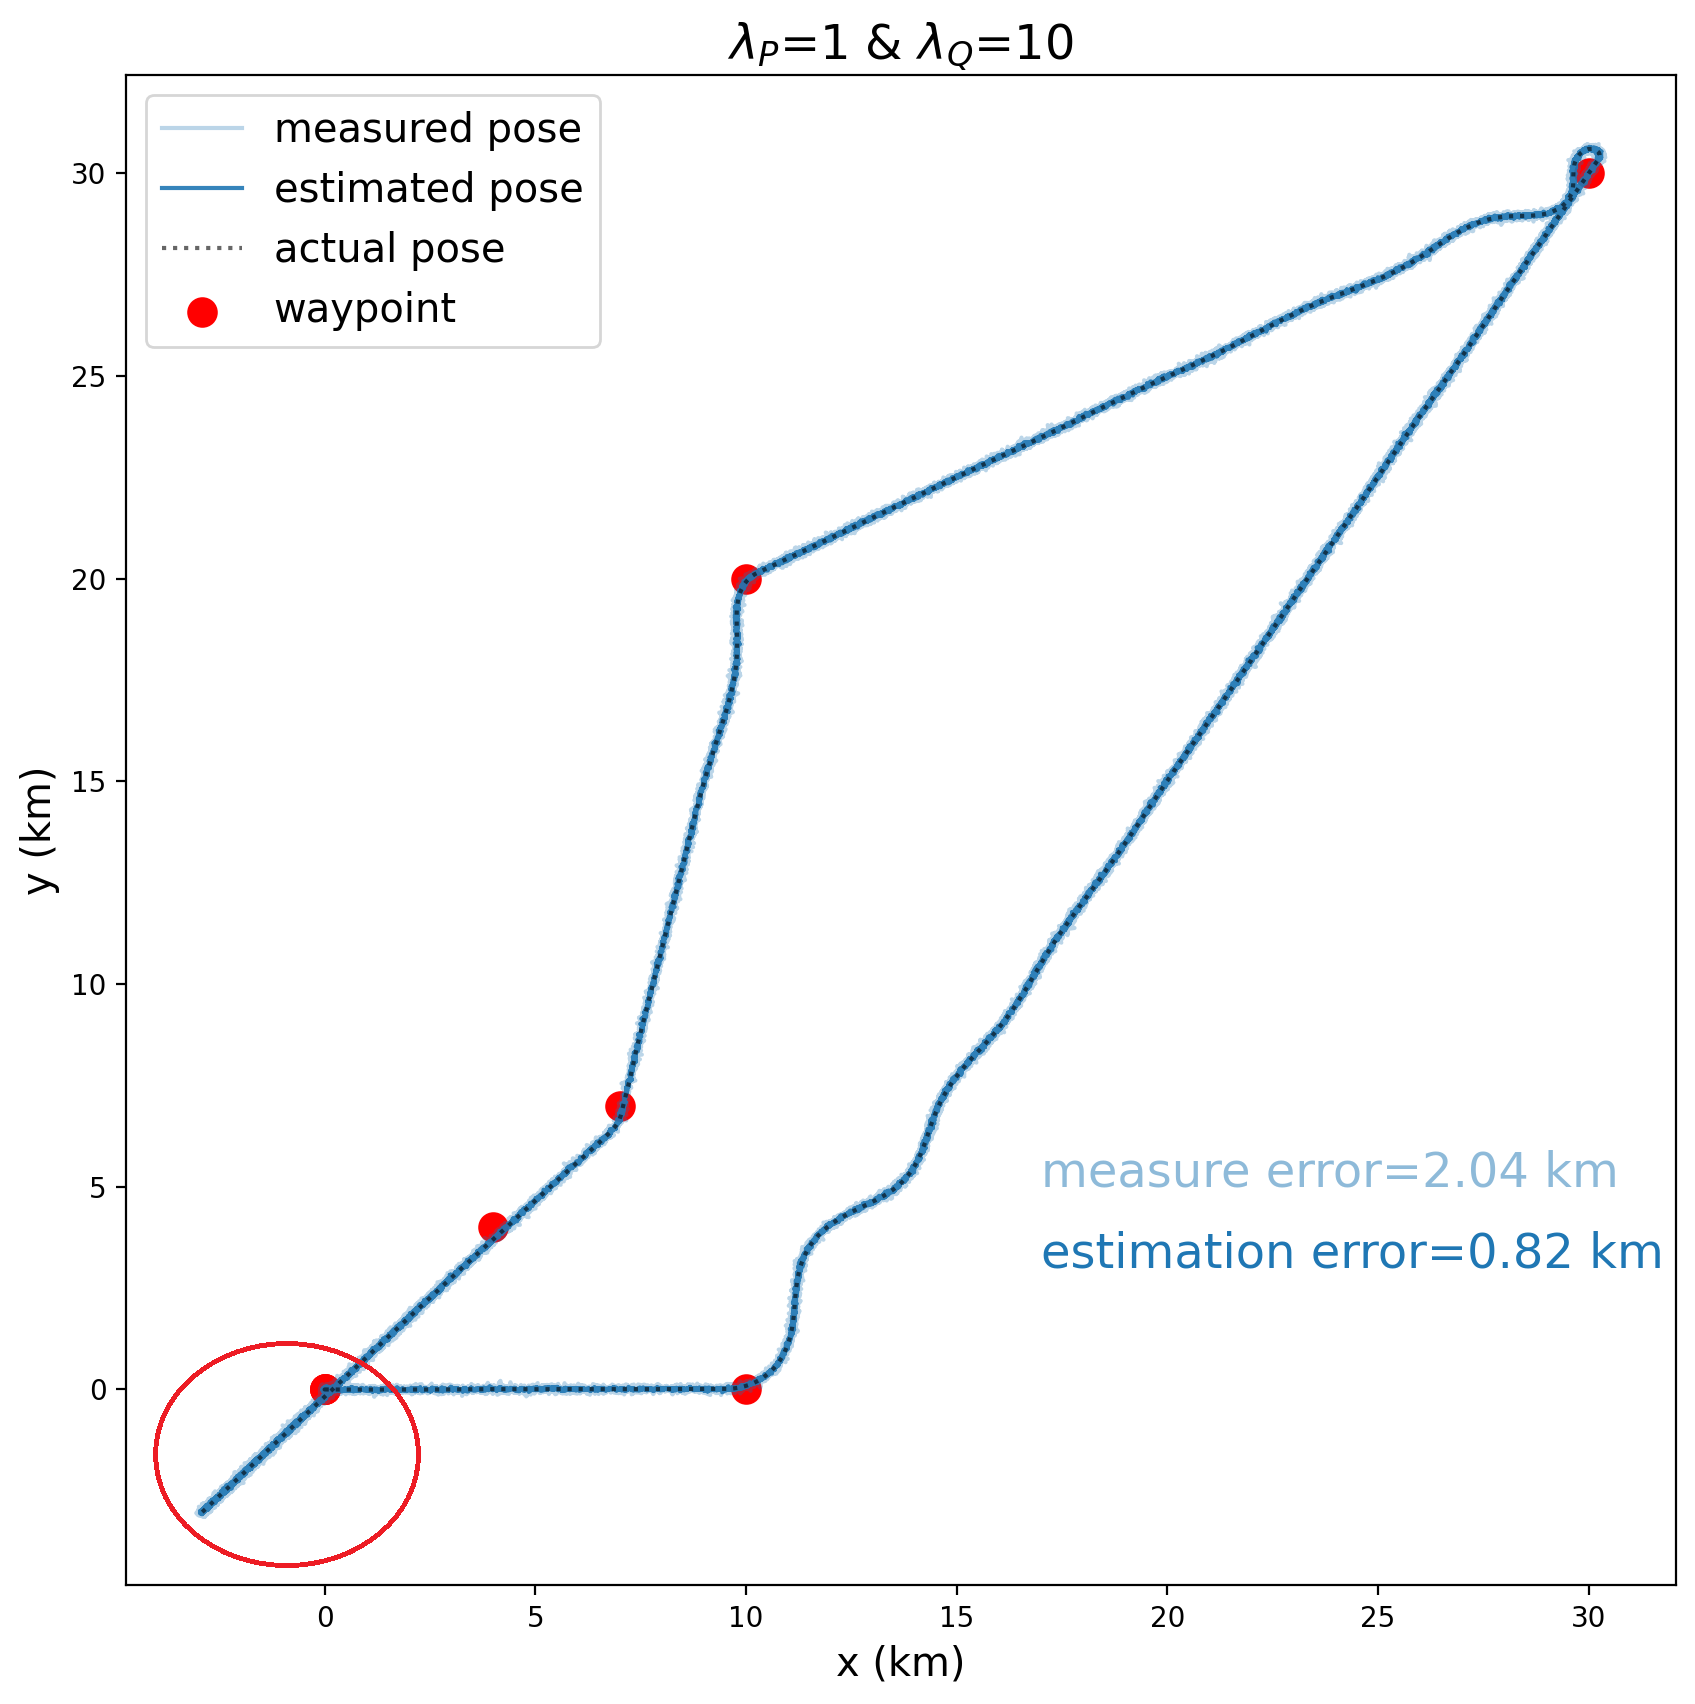
\includegraphics[width=\linewidth]{figures/estimate_P1_Q10_2d.png}
 		\caption{$\lambda_Q=1\:\&\:\lambda_R=10$}
 	\end{subfigure} 
 	\hfill
 	\begin{subfigure}[t]{0.24\textwidth}
 		\centering
 		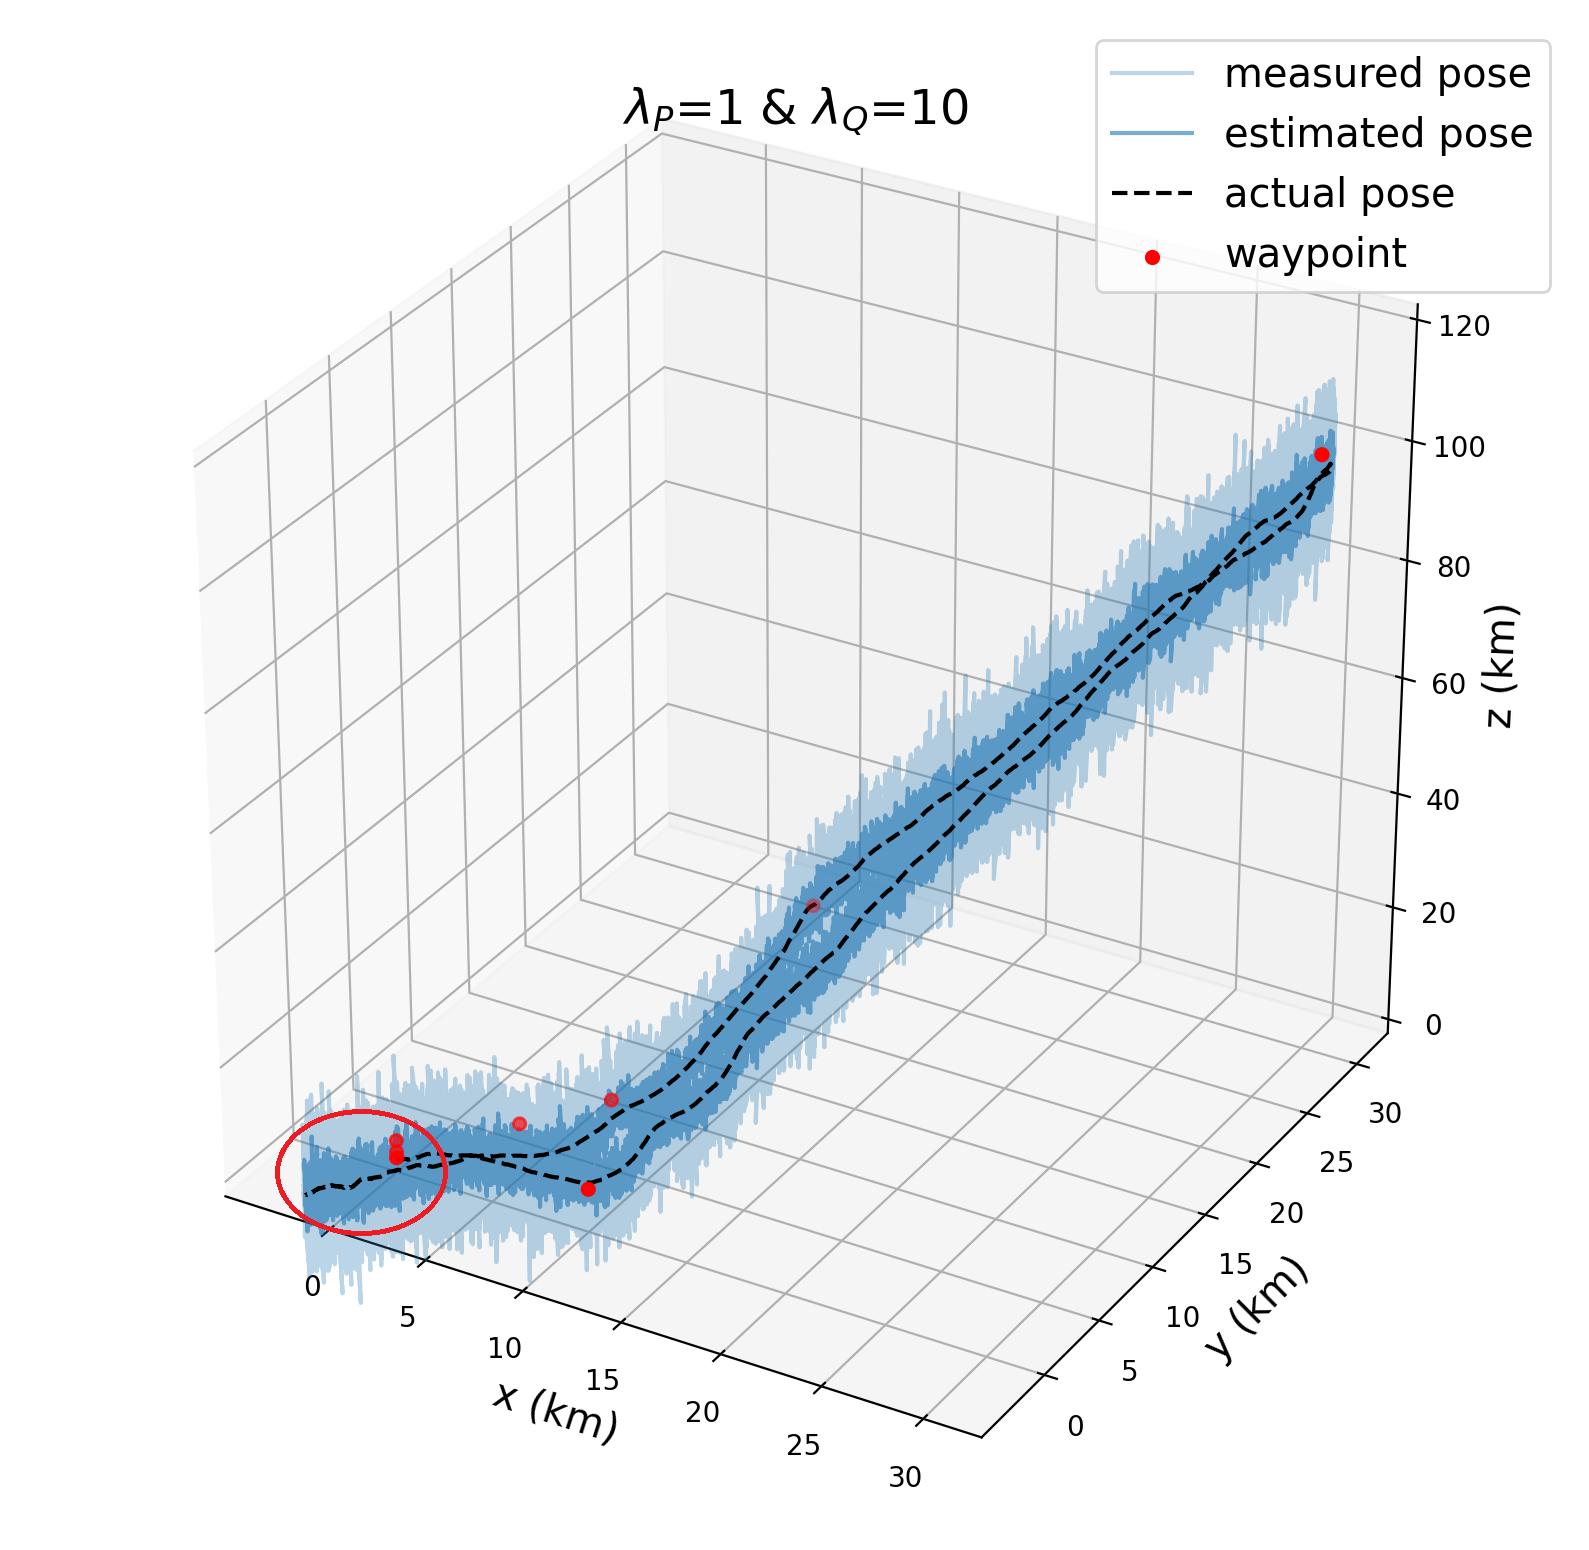
\includegraphics[width=\linewidth]{figures/estimate_P1_Q10_3d.png}
 		\caption{$\lambda_Q=1\:\&\:\lambda_R=10$}
 	\end{subfigure} \\
 	\hfill
 	\begin{subfigure}[t]{0.24\textwidth}
 		\centering
 		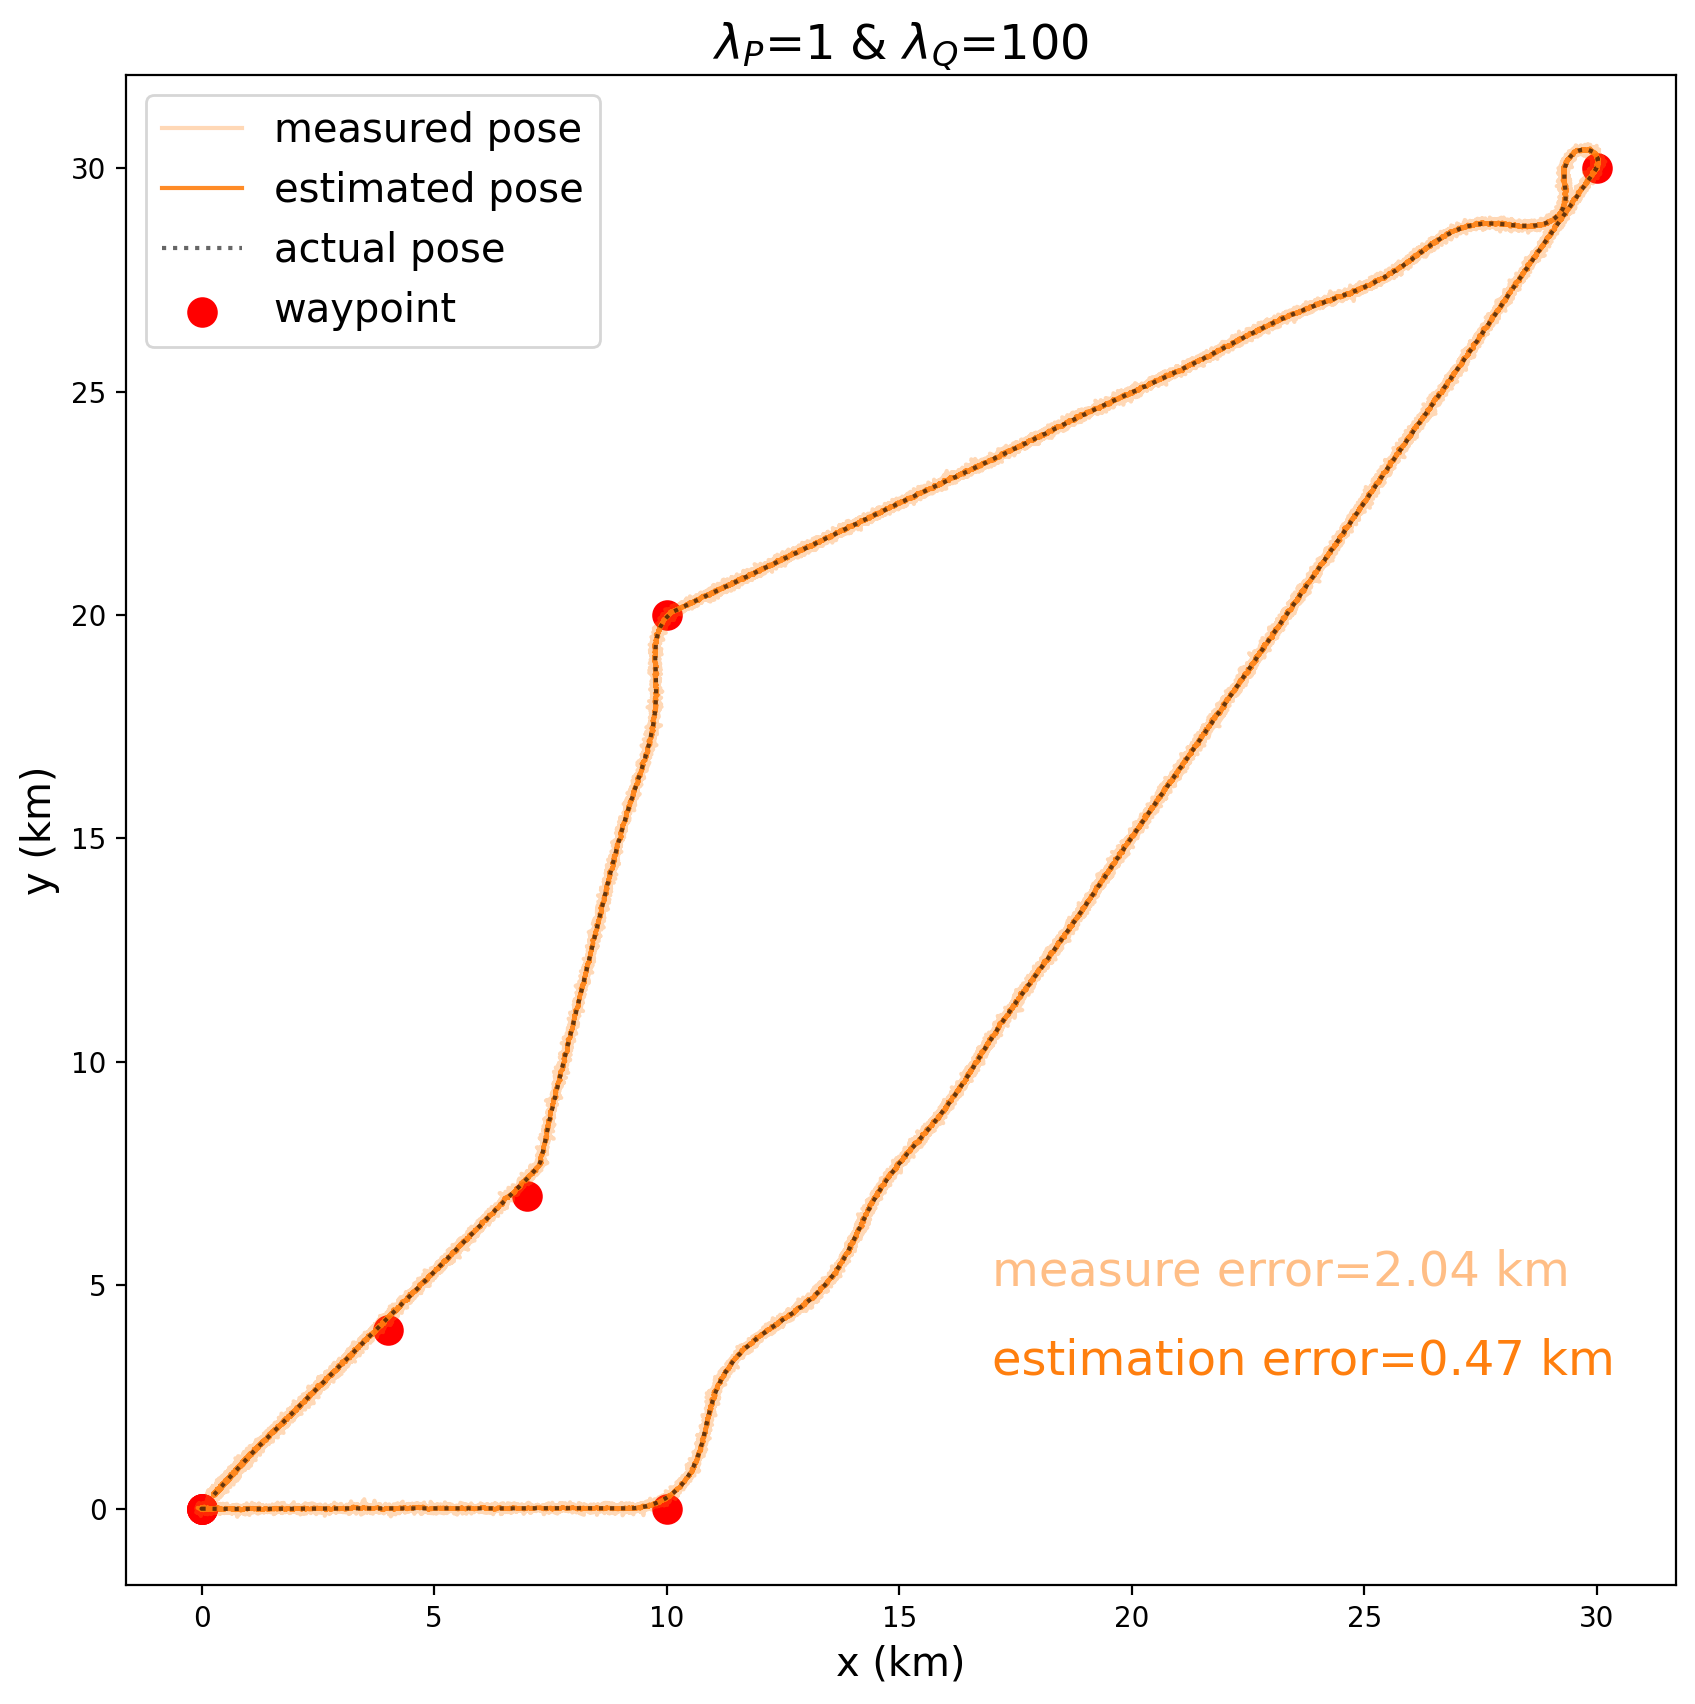
\includegraphics[width=\linewidth]{figures/estimate_P1_Q100_2d.png}
 		\caption{$\lambda_Q=1\:\&\:\lambda_R=10$}
 	\end{subfigure} 
 	\hfill
 	\begin{subfigure}[t]{0.24\textwidth}
 		\centering
 		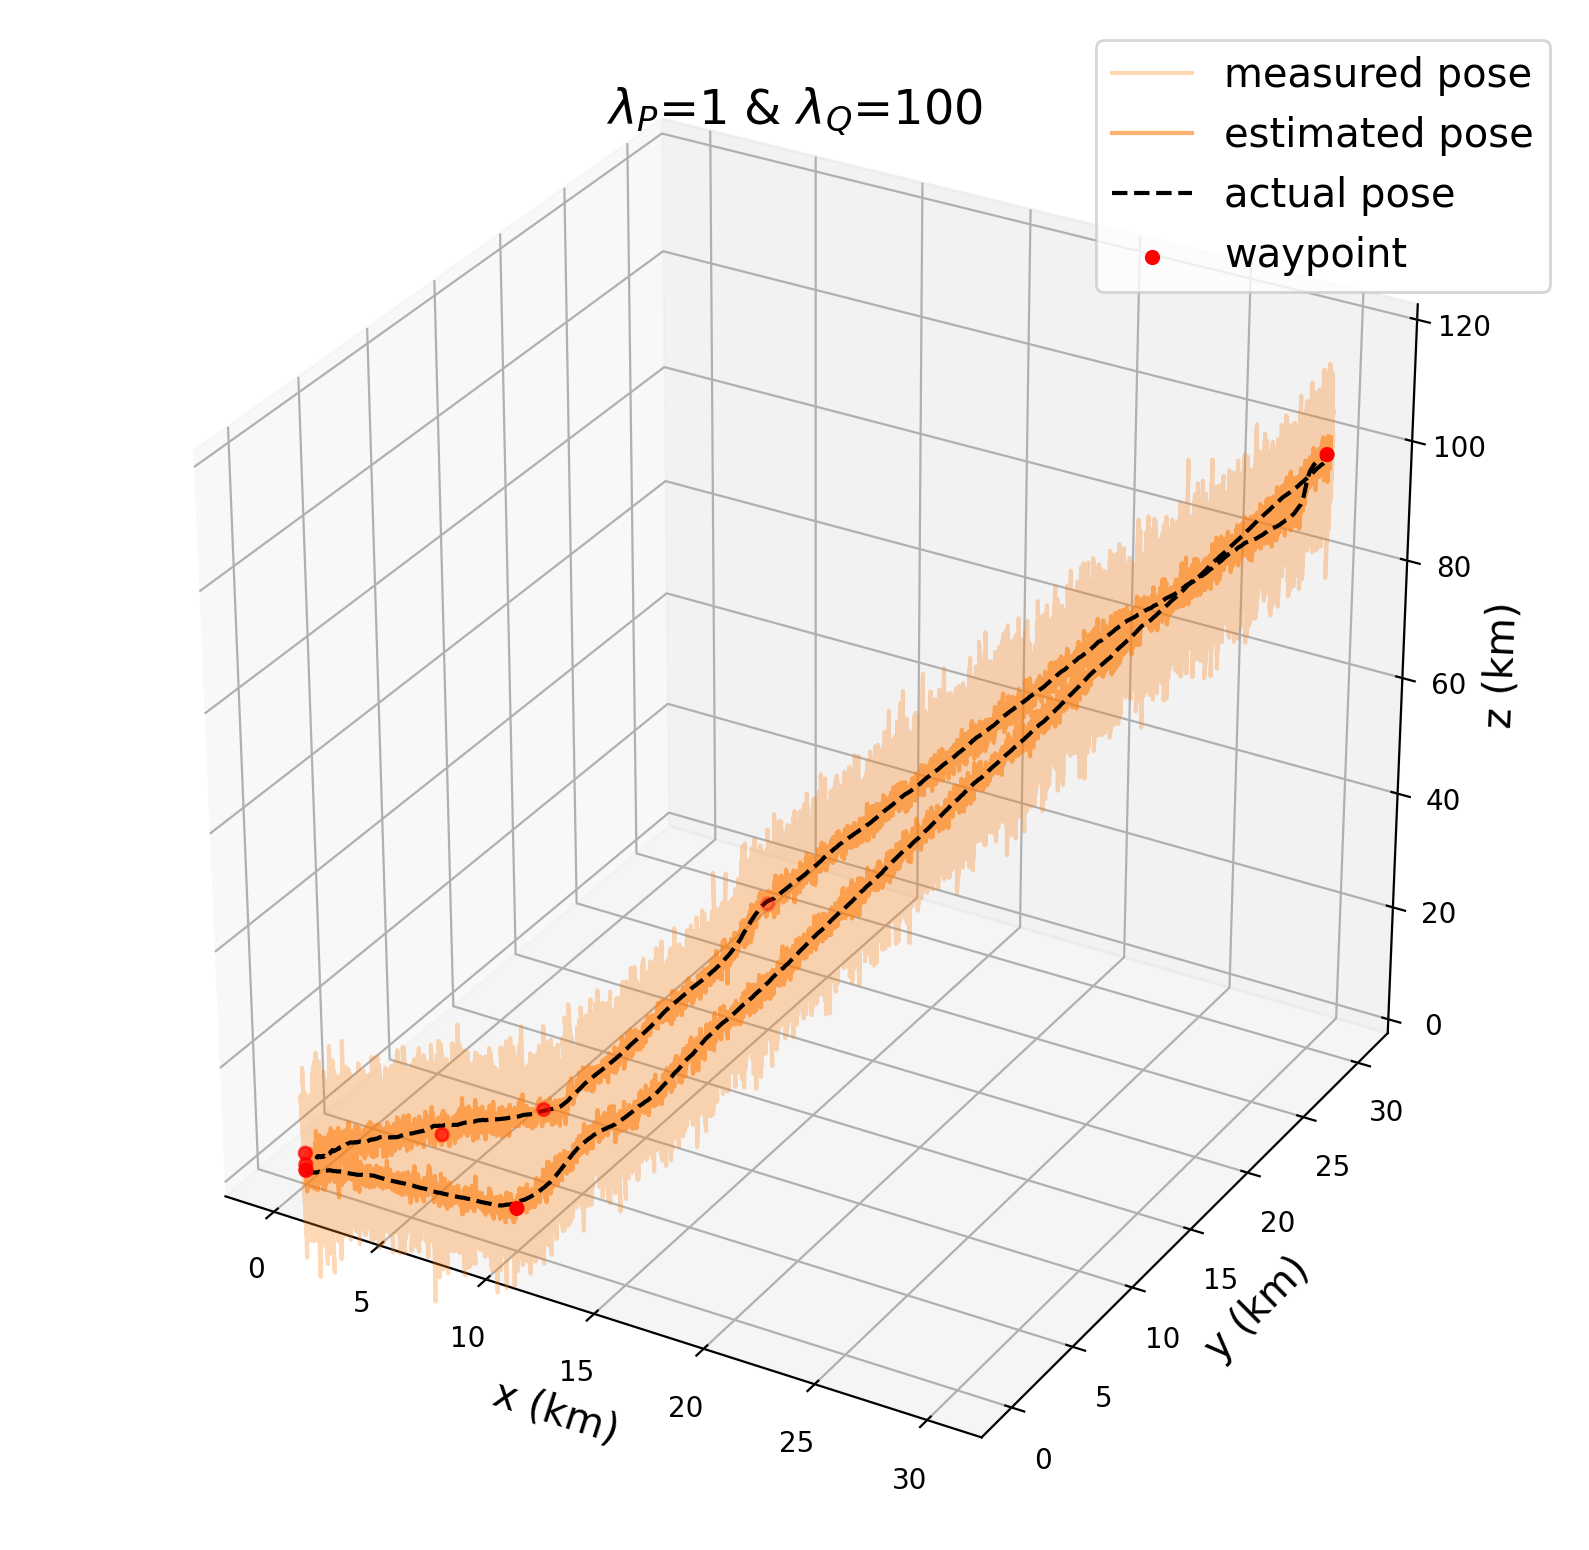
\includegraphics[width=\linewidth]{figures/estimate_P1_Q100_3d.png}
 		\caption{$\lambda_Q=1\:\&\:\lambda_R=10$}
 	\end{subfigure} \\
 	\hfill
 	\begin{subfigure}[t]{0.24\textwidth}
 		\centering
 		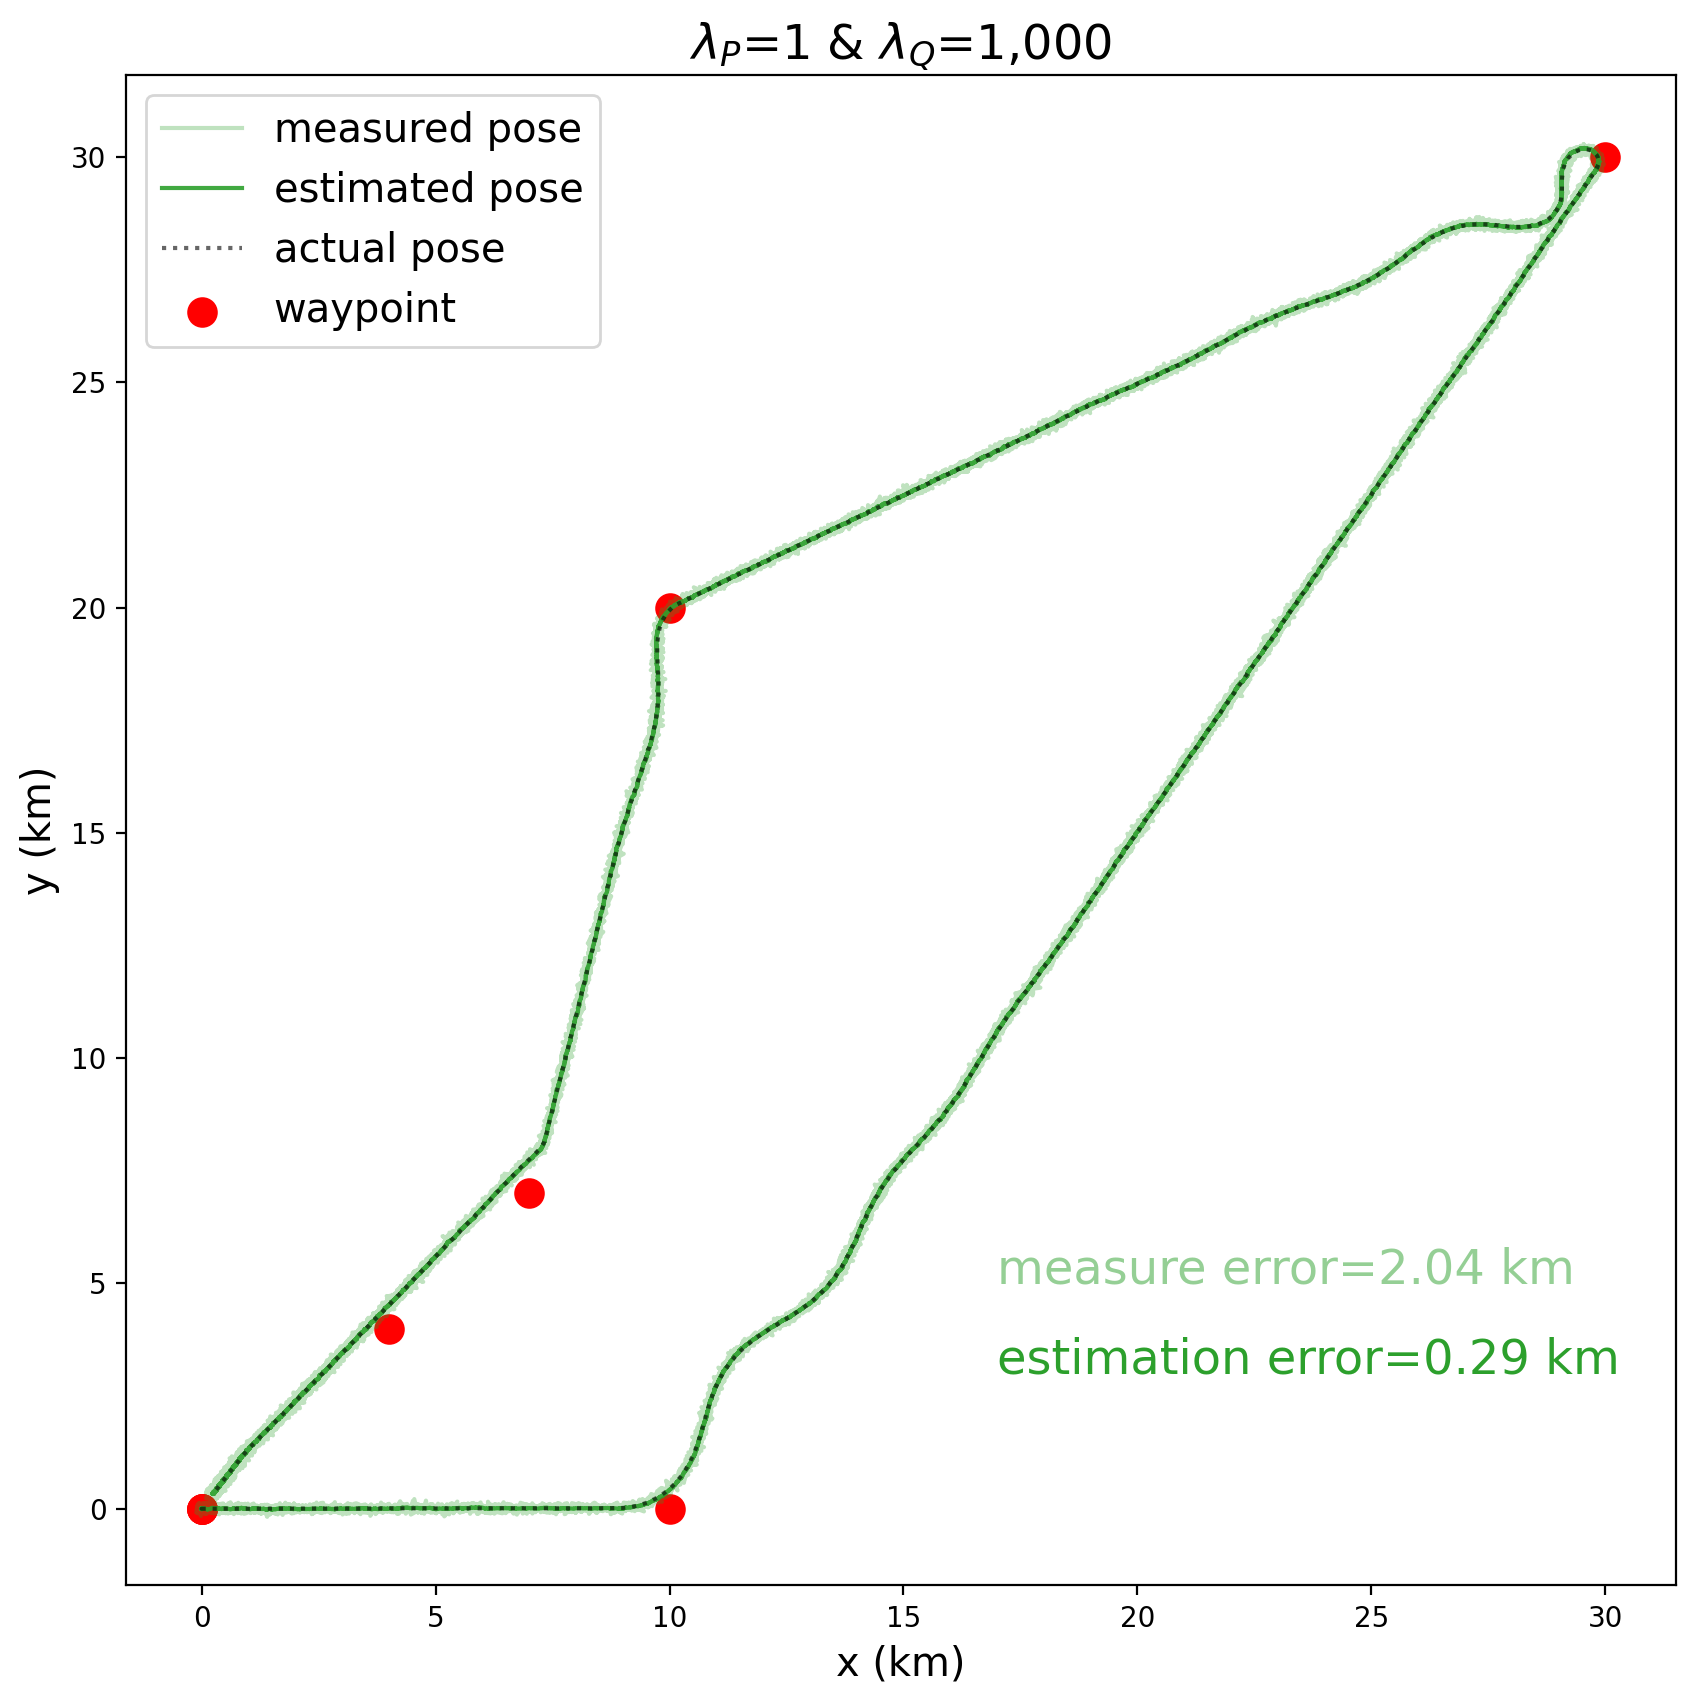
\includegraphics[width=\linewidth]{figures/estimate_P1_Q1000_2d.png}
 		\caption{$\lambda_Q=1\:\&\:\lambda_R=10$}
 	\end{subfigure} 
 	\hfill
 	\begin{subfigure}[t]{0.24\textwidth}
 		\centering
 		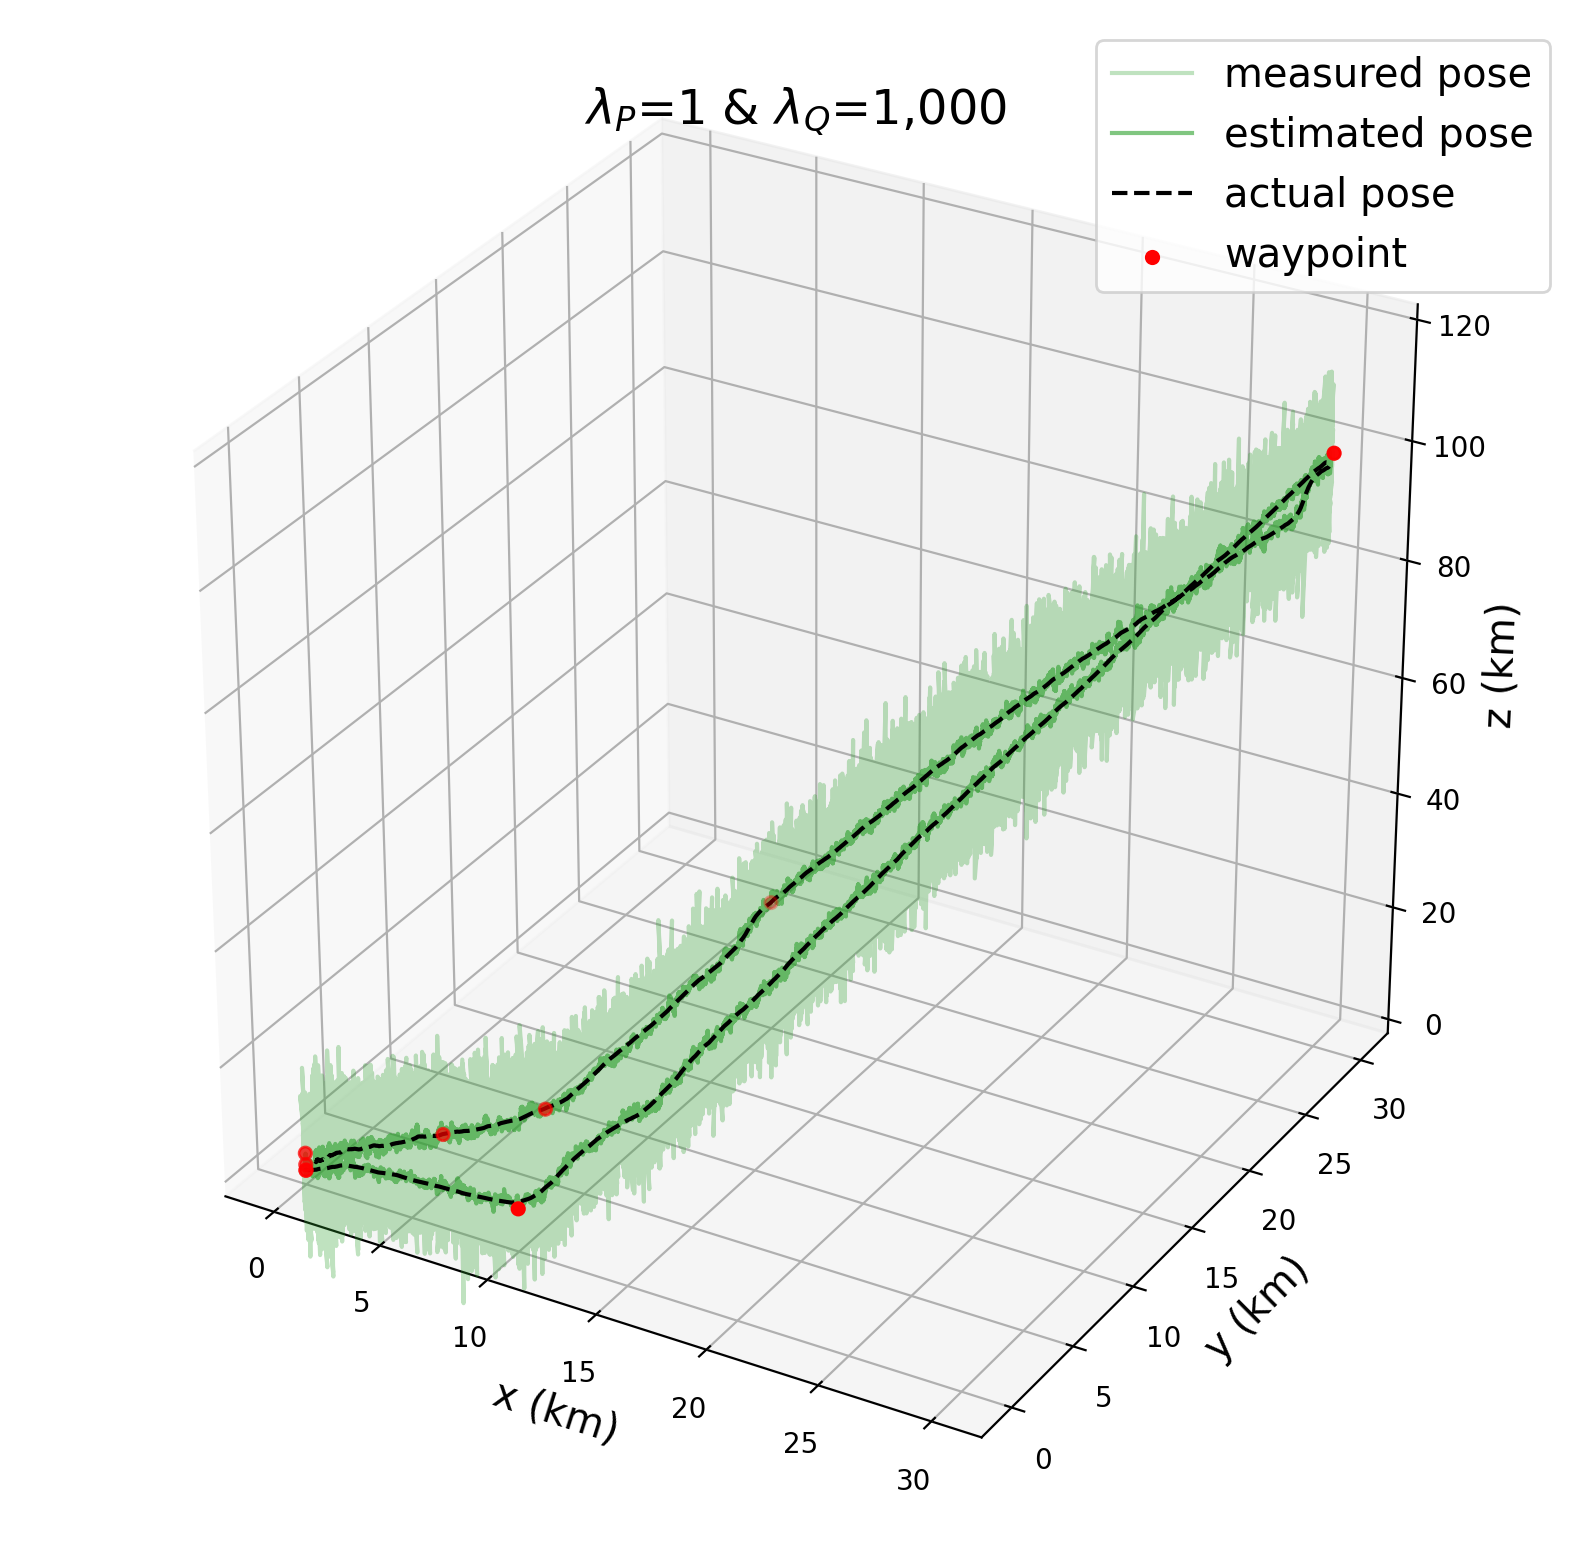
\includegraphics[width=\linewidth]{figures/estimate_P1_Q1000_3d.png}
 		\caption{$\lambda_Q=1\:\&\:\lambda_R=10$}
 	\end{subfigure} 
 	
 	\caption{Two-dimensional plot (left column: a, c, and e) and three-dimensional plot (right column: b, d, and f) of the measured trajectories and the estimated trajectories with $\lambda_Q=1\:\&\:\lambda_R=10$ (blue), $\lambda_Q=1\:\&\:\lambda_R=100$ (orange), and $\lambda_Q=1\:\&\:\lambda_R=1,000$ (green).}
 	
 	\label{fig:exp_QR}
 \end{figure}
  
 The result of the first experiment is shown in Fig.~\ref{fig:exp_QR}. The figure presents that, due to a strong measurement noise, using large $\lambda_R$ improves the estimation performance. Without state estimation, the root-mean-square error of the measured trajectory is 2.04 km in all cases. Using $\lambda_Q=1\:\&\:\lambda_R=1,000$ can lower the root-mean-square error to 0.29 km (i.e., 86\% reduction). Interestingly, if $\lambda_Q=1\:\&\:\lambda_R=1,000$, the error is relatively high, or rather 0.82. Consequently, the spaceship misses the acceptance sphere and does not stop at stopping point, as highlighted by red circles in Fig.~\ref{fig:exp_QR}(a,b). 
 

\subsection{Experiment 2: Control}
\label{sec:exp_control}

With $\lambda_Q=1\:\&\:\lambda_R=1,000$, the second experiment compares three values $K_d$. Those are $K_d=500$ (blue), $K_d=1,000$ (orange), and $K_d=1,500$ (green). Note that, in this experiment, $K_p$ representing convergence time is fixed as 1,000 during the comparison. increasing $K_p$ will increase the speed of the spaceship.  During this, the guidance parameter $\eta_\Delta$ and $\eta_e$ are still fixed at 100 and 0.1.

\begin{figure}[h]
	\centering
	\begin{subfigure}[t]{0.24\textwidth}
		\centering
		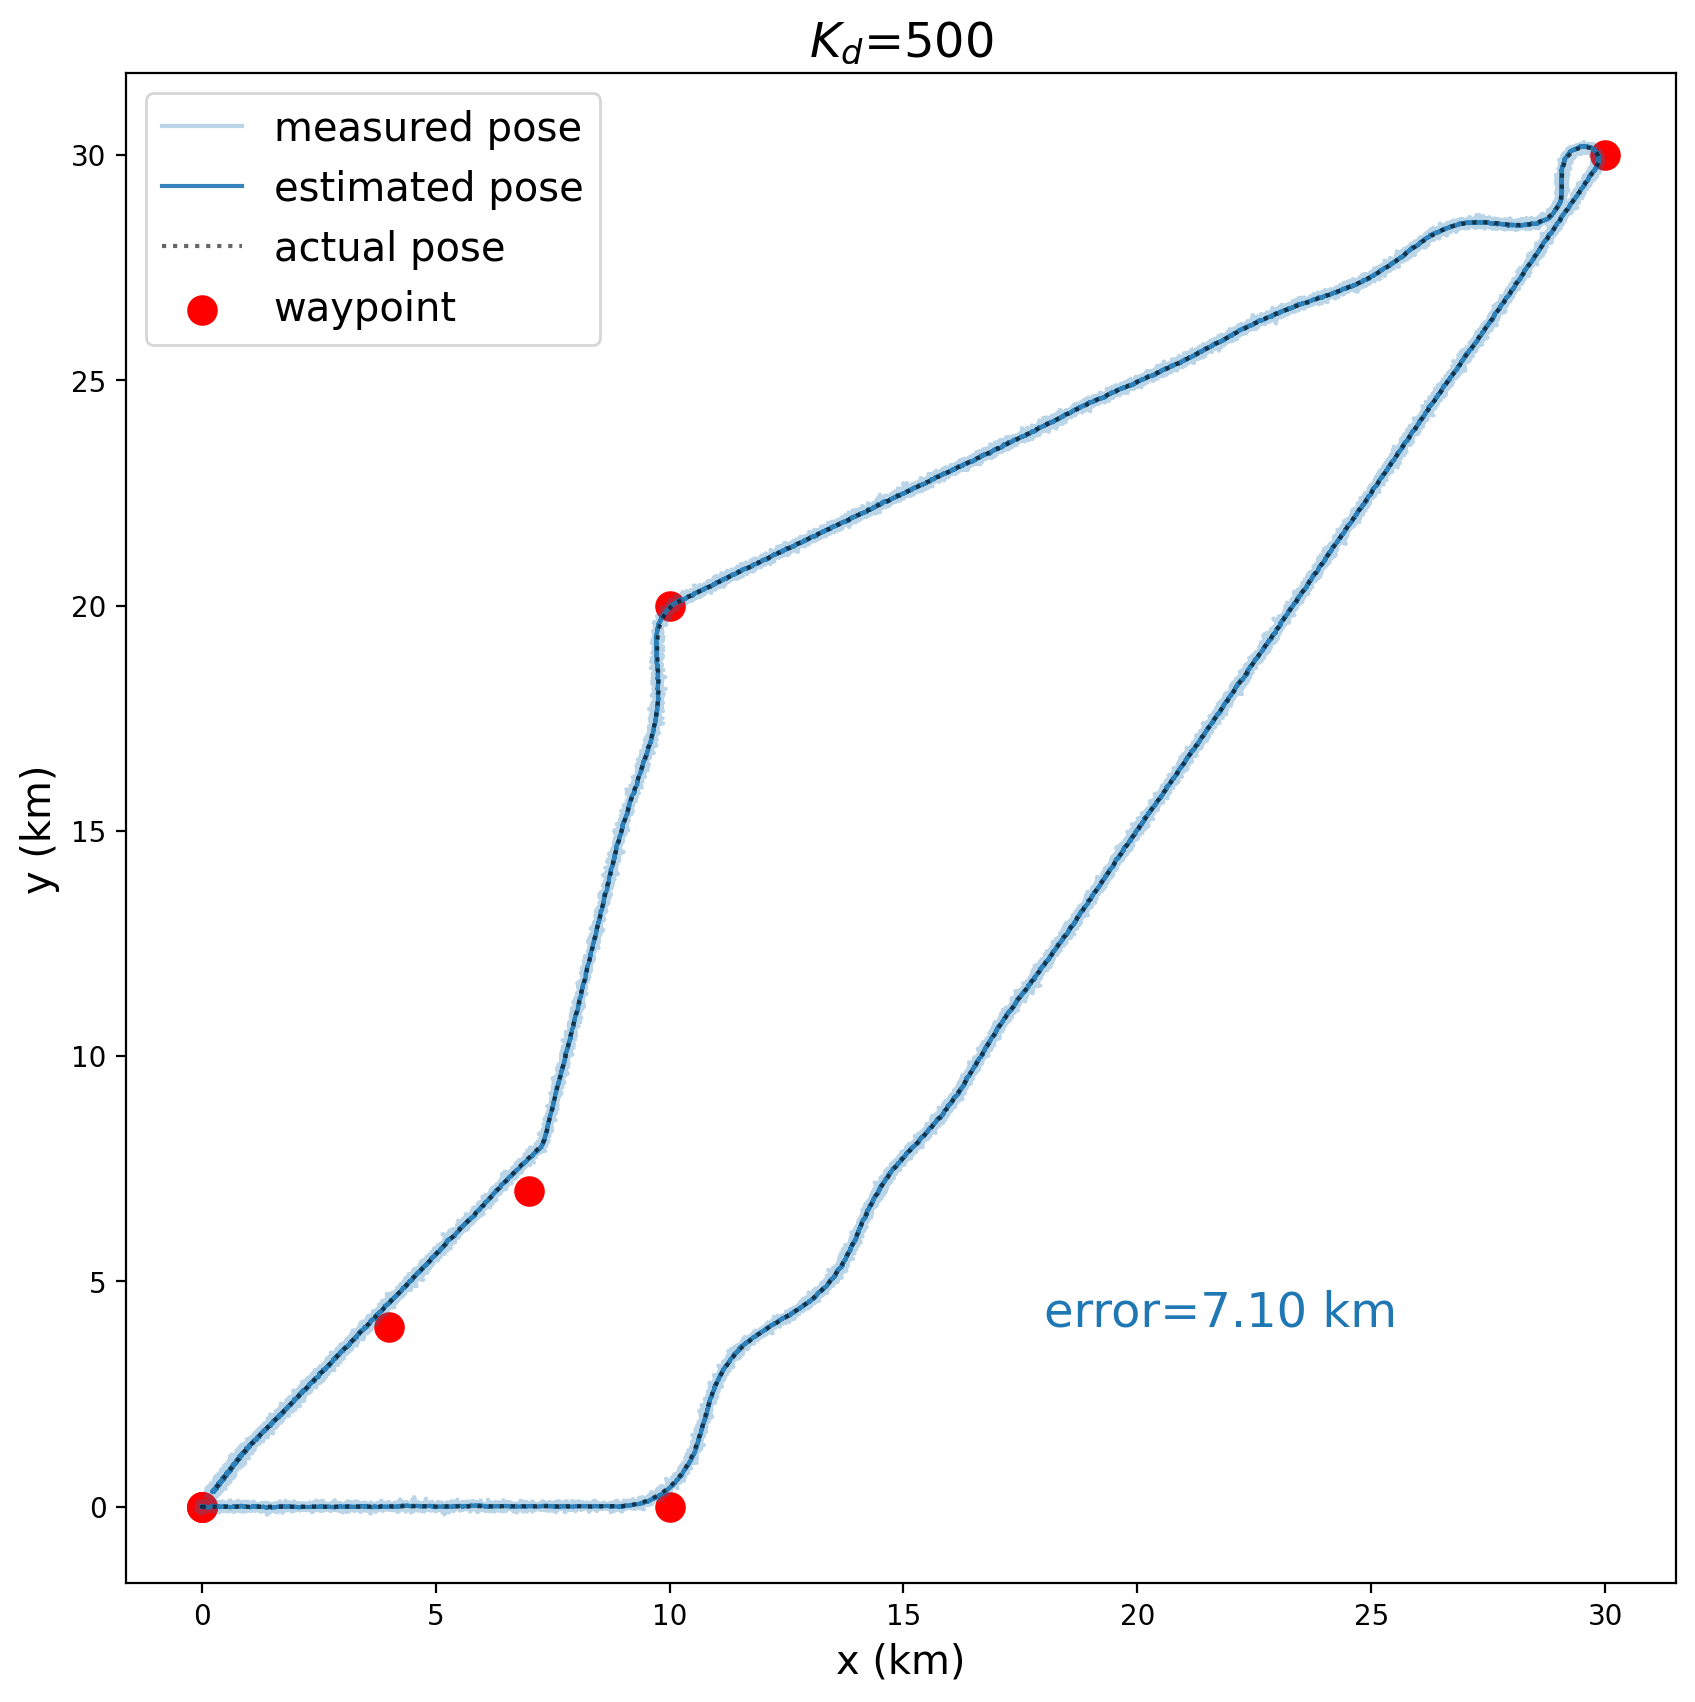
\includegraphics[width=\linewidth]{figures/Dgain_D05_2d.png}
		\caption{$K_d=500$}
	\end{subfigure} 
	\hfill
	\begin{subfigure}[t]{0.24\textwidth}
		\centering
		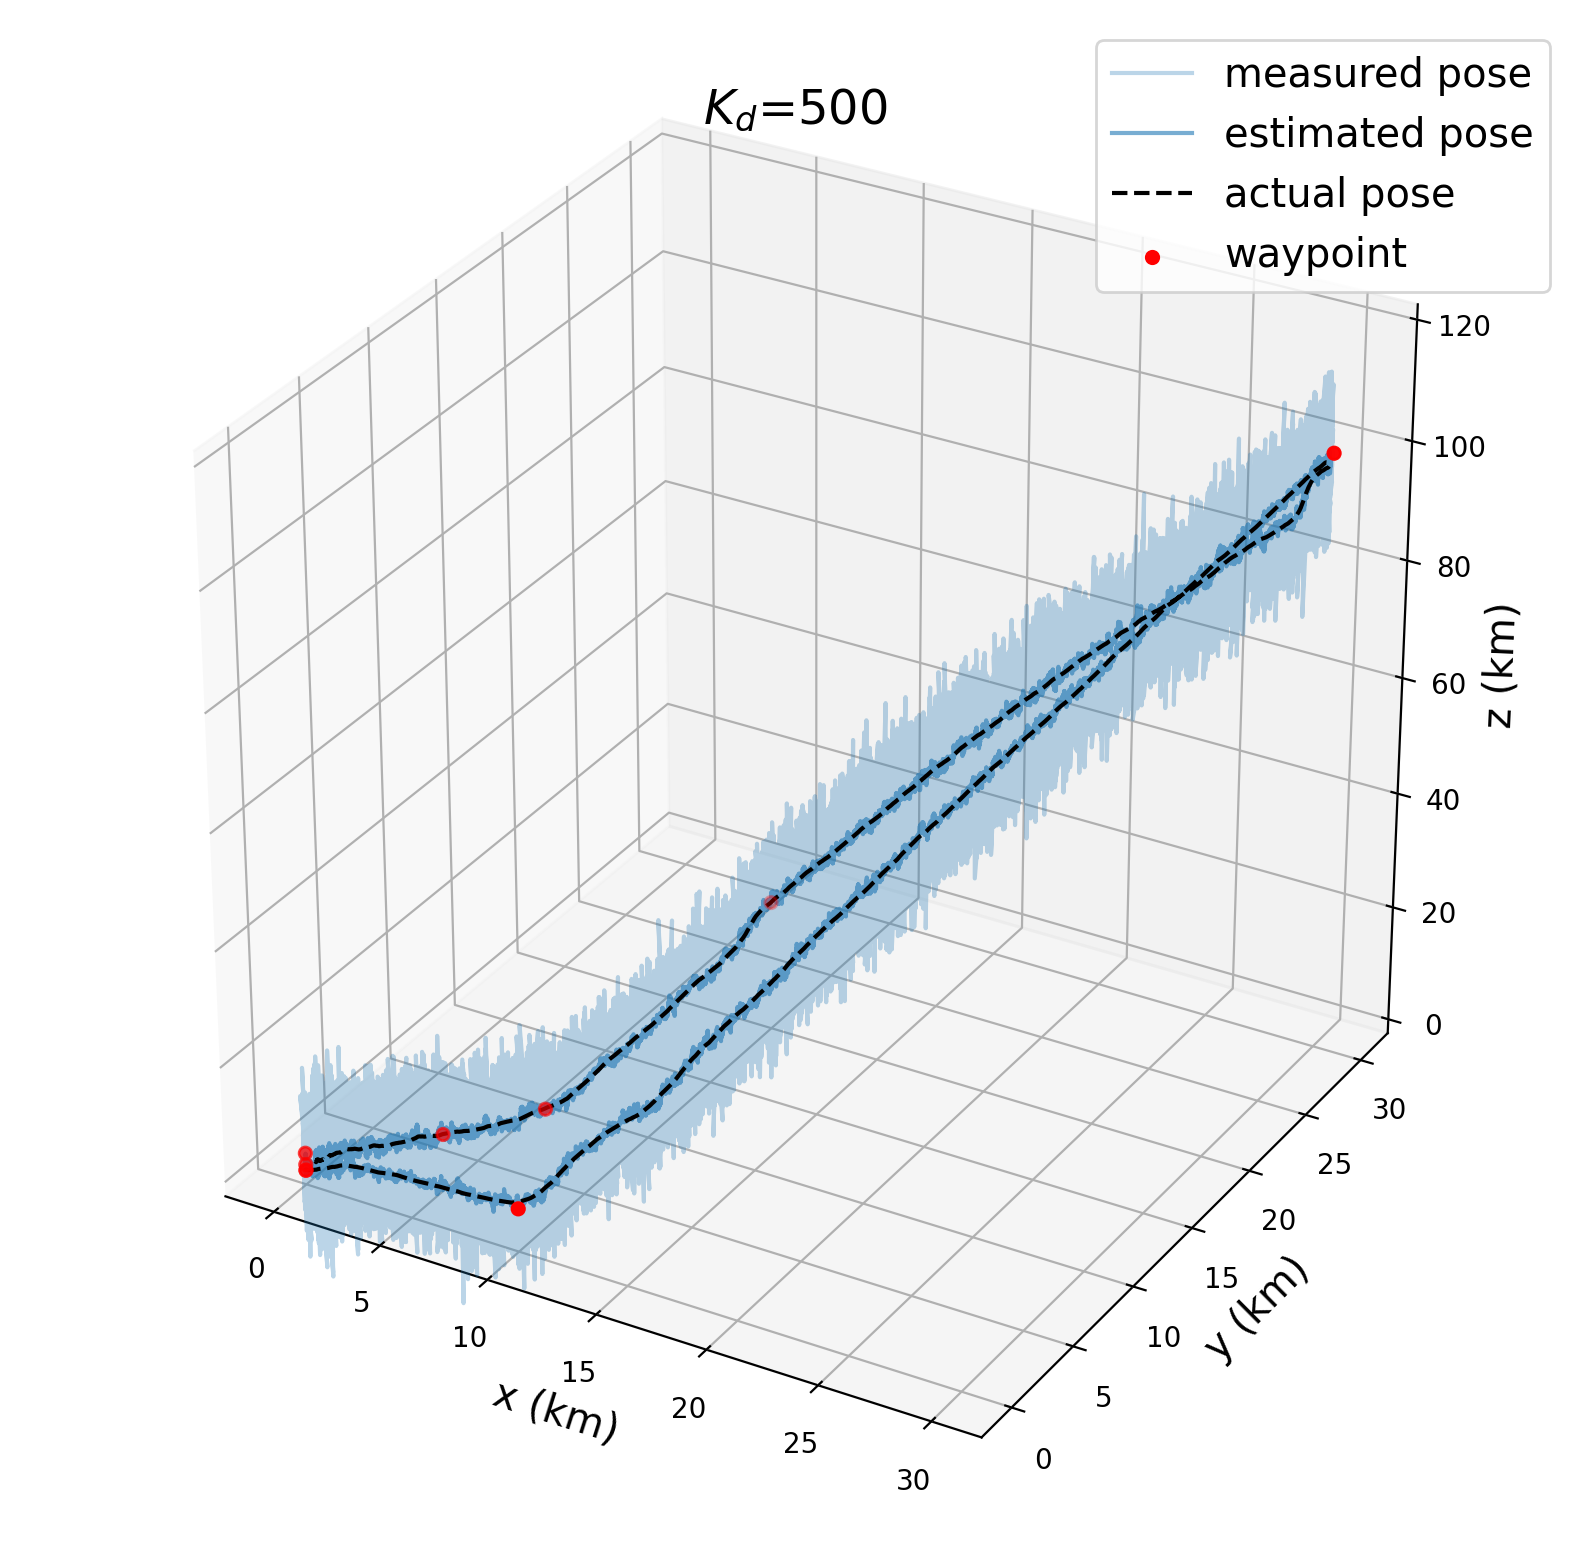
\includegraphics[width=\linewidth]{figures/Dgain_D05_3d.png}
		\caption{$K_d=500$}
	\end{subfigure} \\
	\hfill
	\begin{subfigure}[t]{0.24\textwidth}
		\centering
		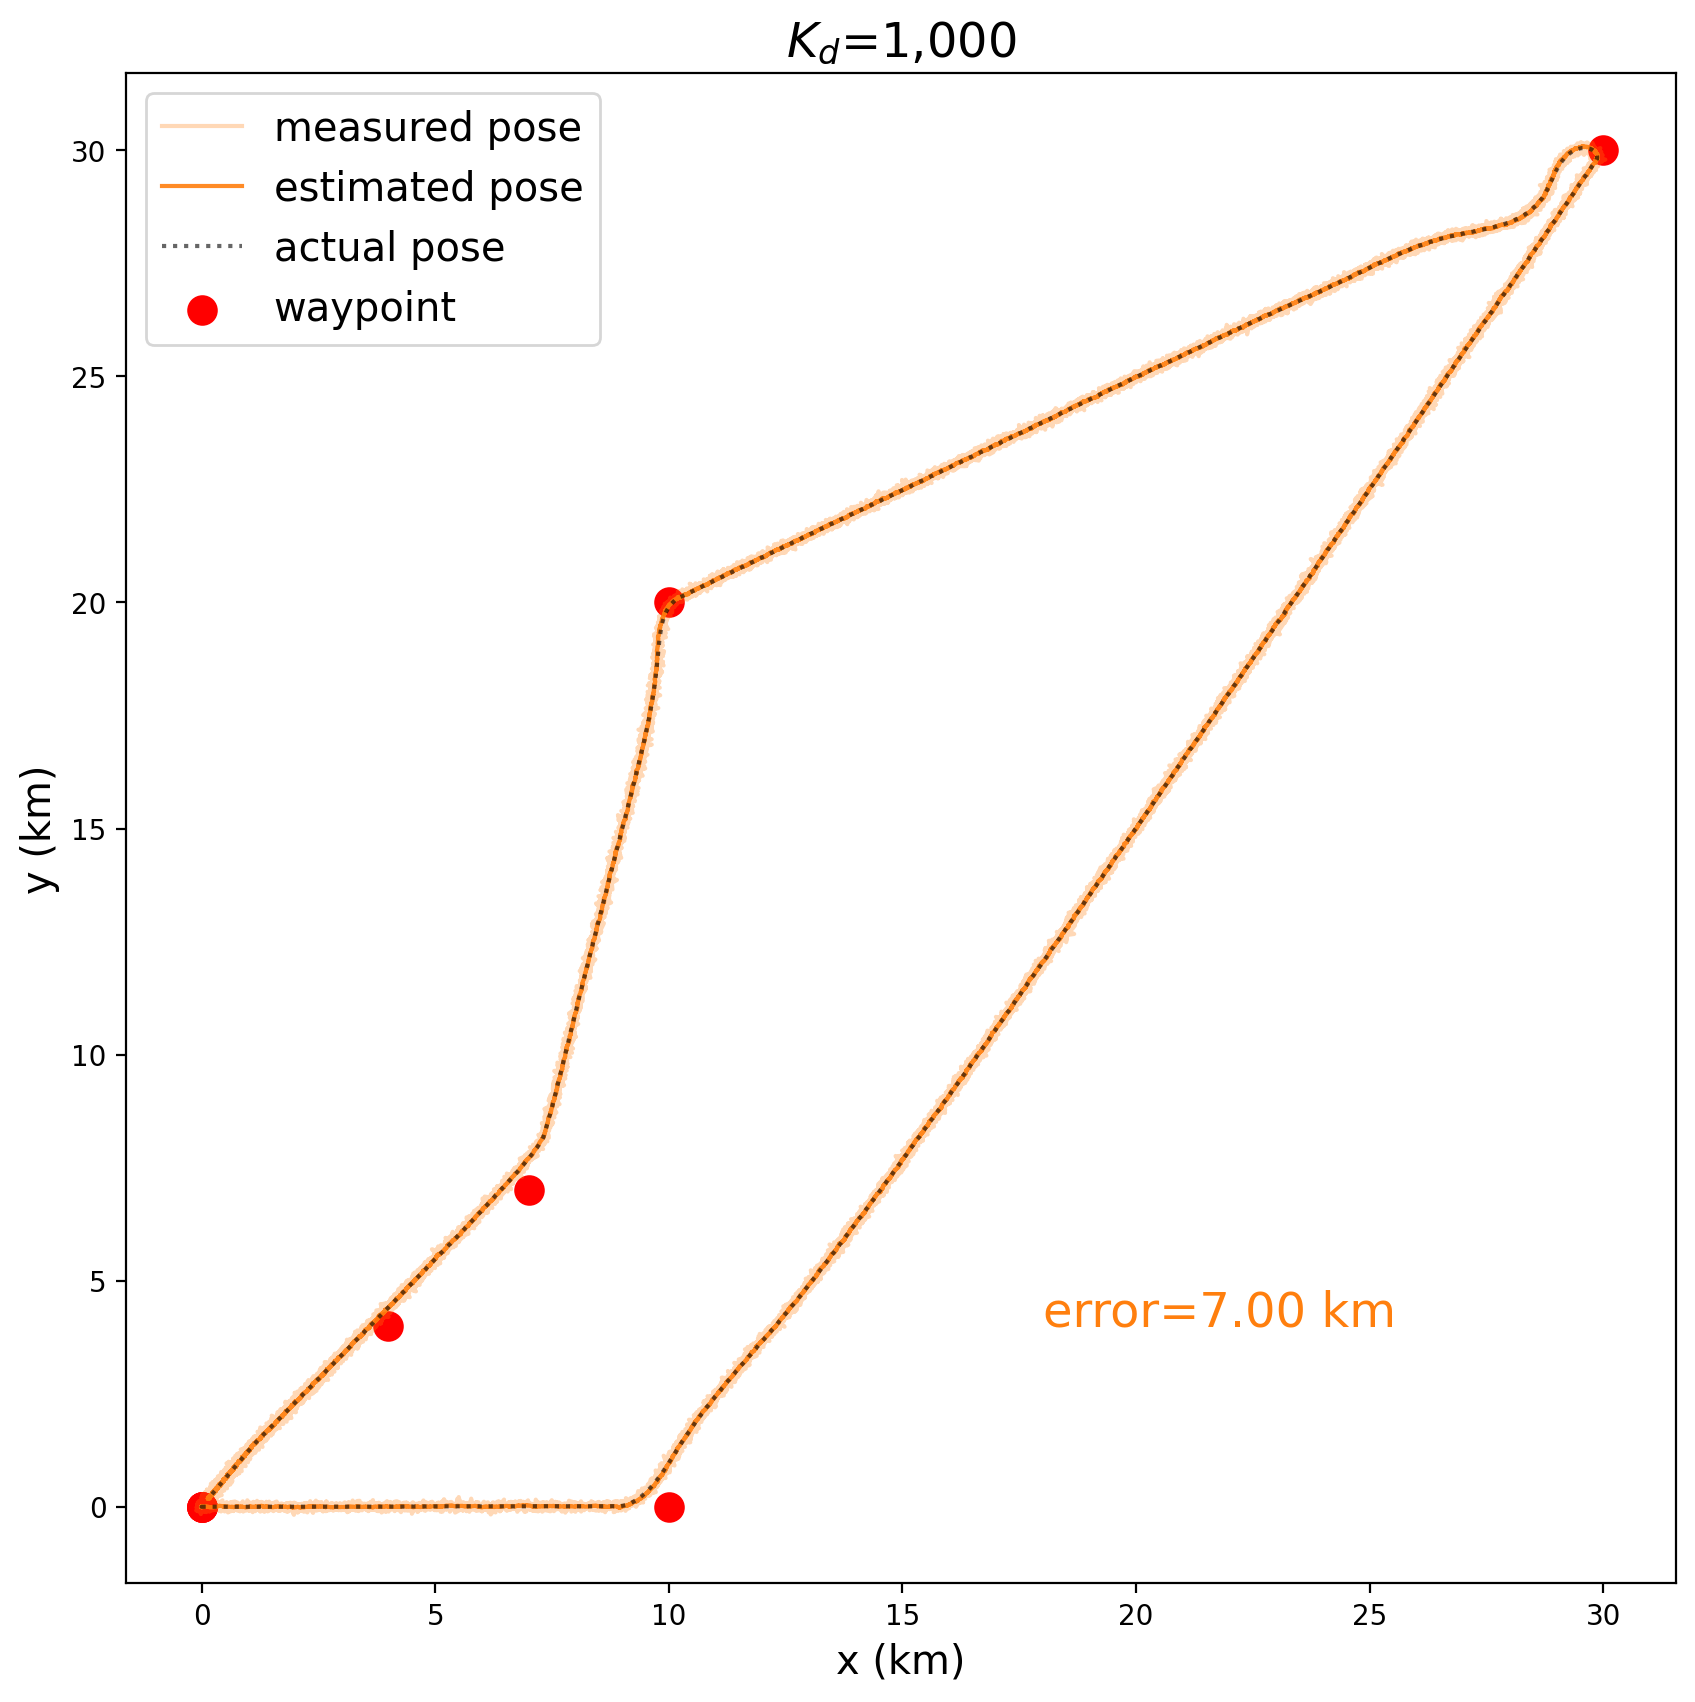
\includegraphics[width=\linewidth]{figures/Dgain_D10_2d.png}
		\caption{$K_d=100$}
	\end{subfigure} 
	\hfill
	\begin{subfigure}[t]{0.24\textwidth}
		\centering
		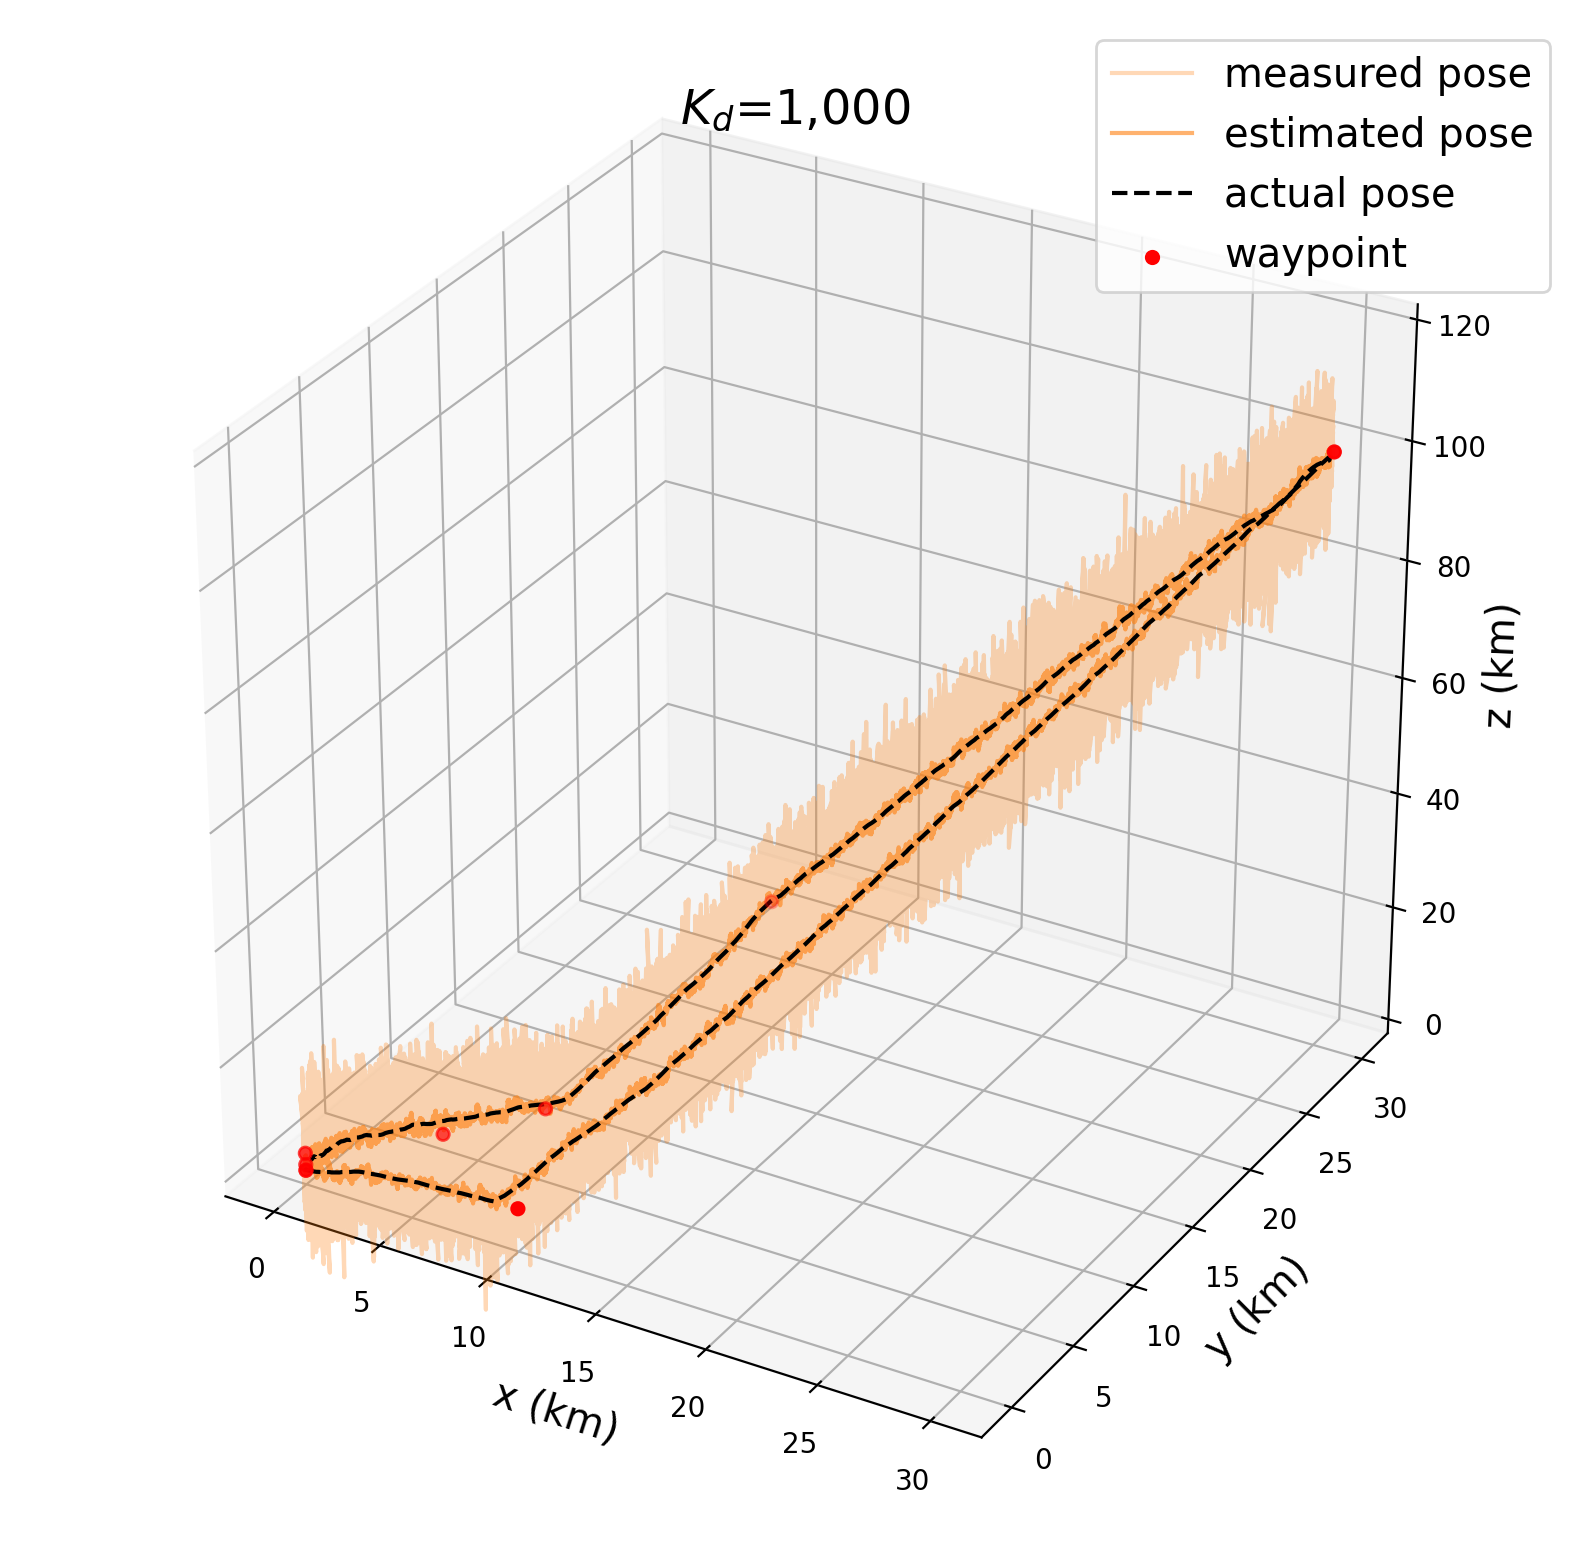
\includegraphics[width=\linewidth]{figures/Dgain_D10_3d.png}
		\caption{$K_d=100$}
	\end{subfigure} \\
	\hfill
	\begin{subfigure}[t]{0.24\textwidth}
		\centering
		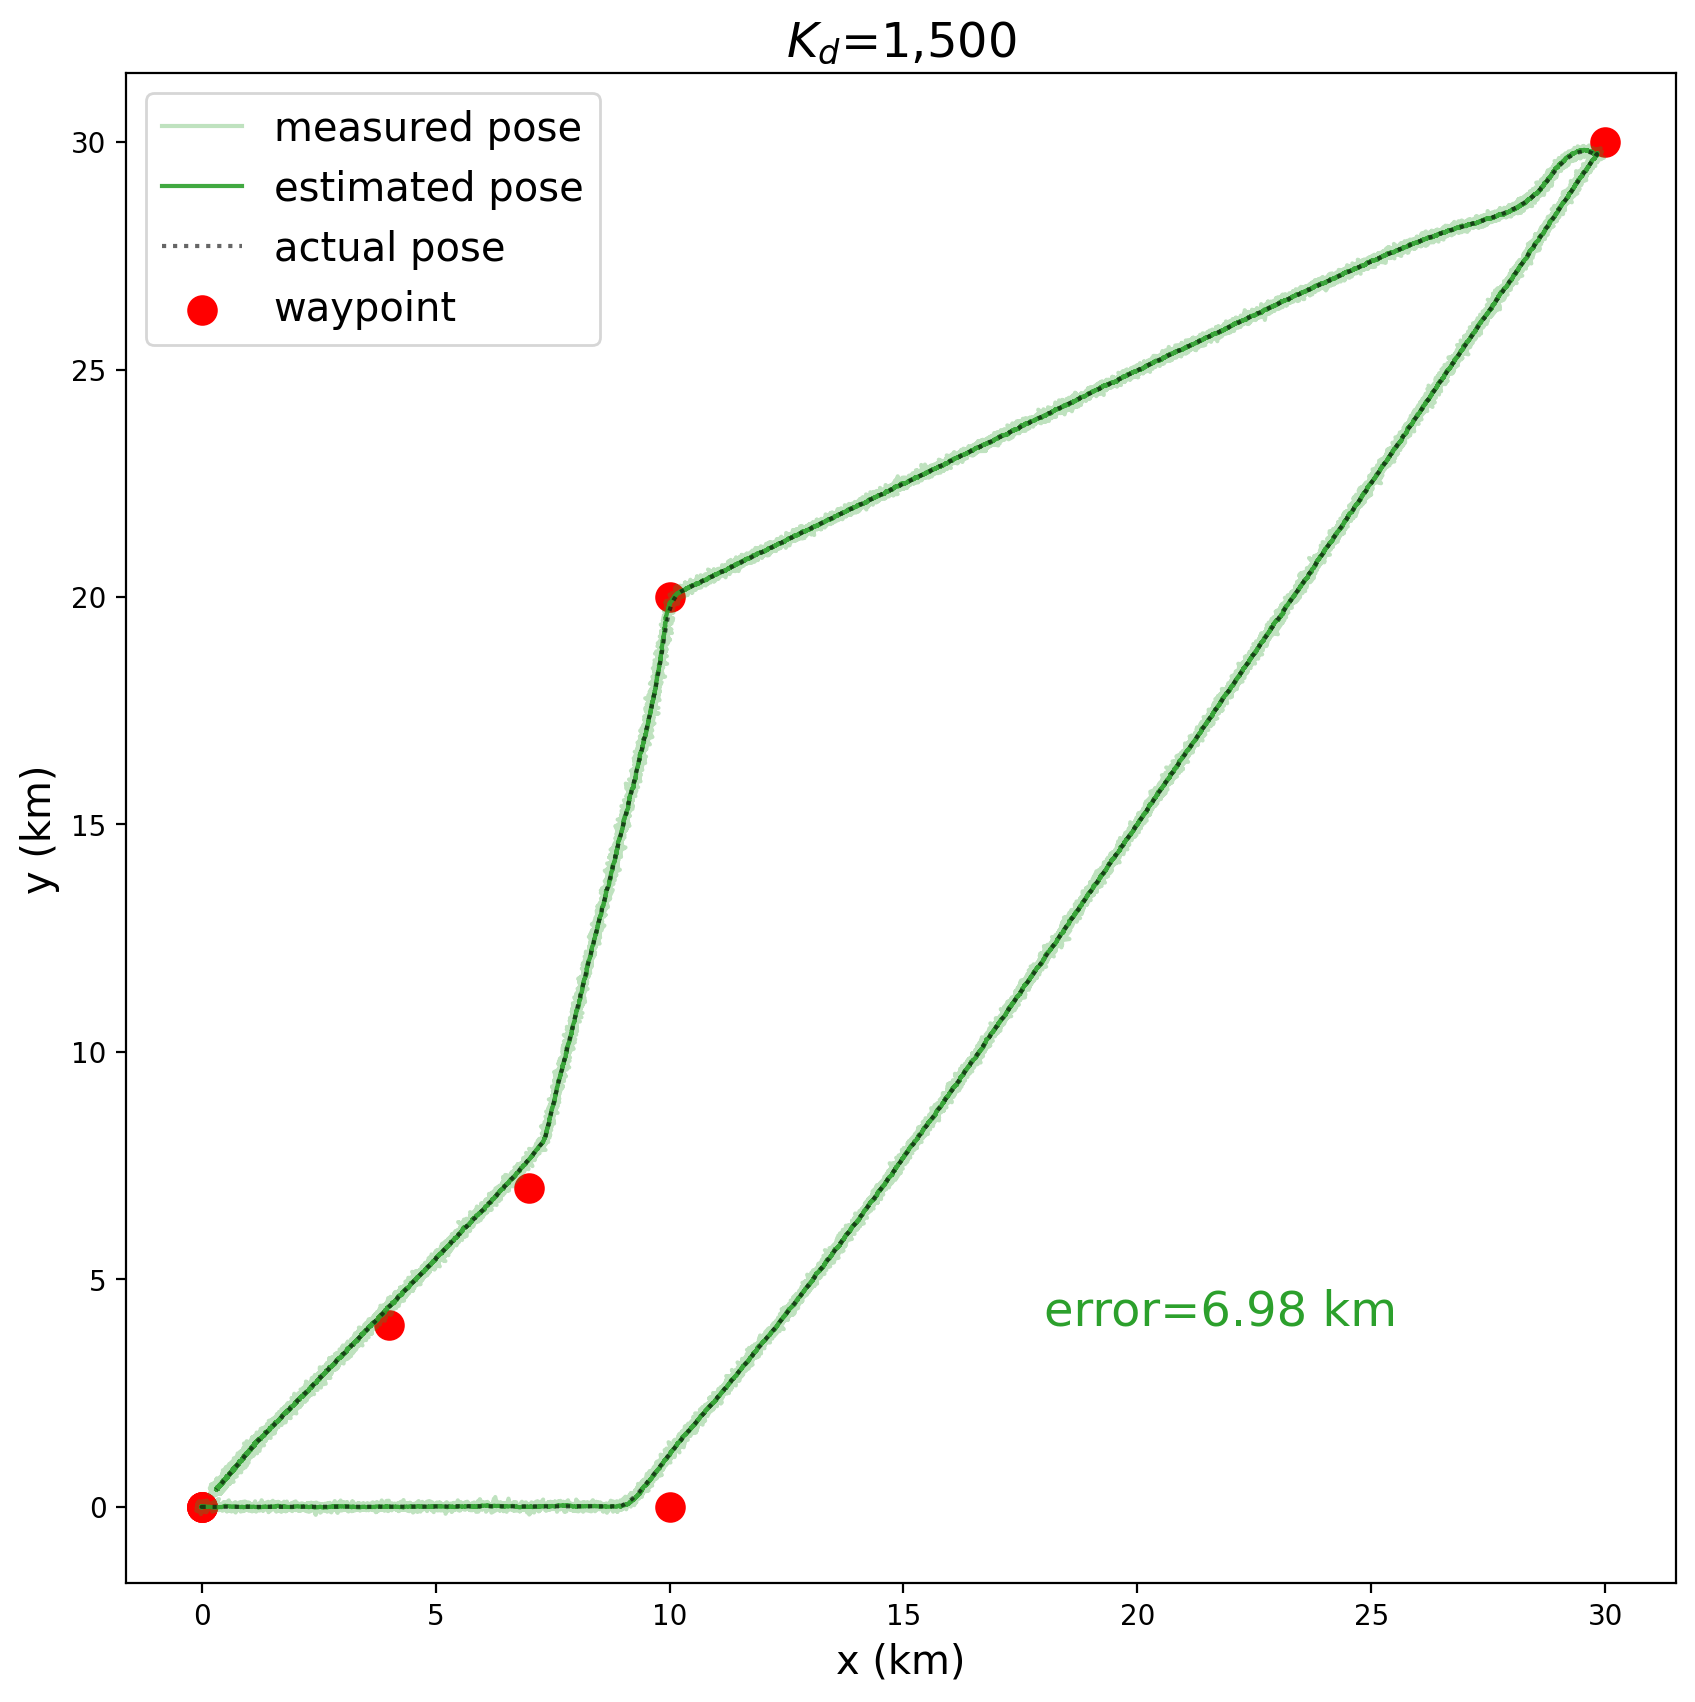
\includegraphics[width=\linewidth]{figures/Dgain_D15_2d.png}
		\caption{$K_d=1,500$}
	\end{subfigure} 
	\hfill
	\begin{subfigure}[t]{0.24\textwidth}
		\centering
		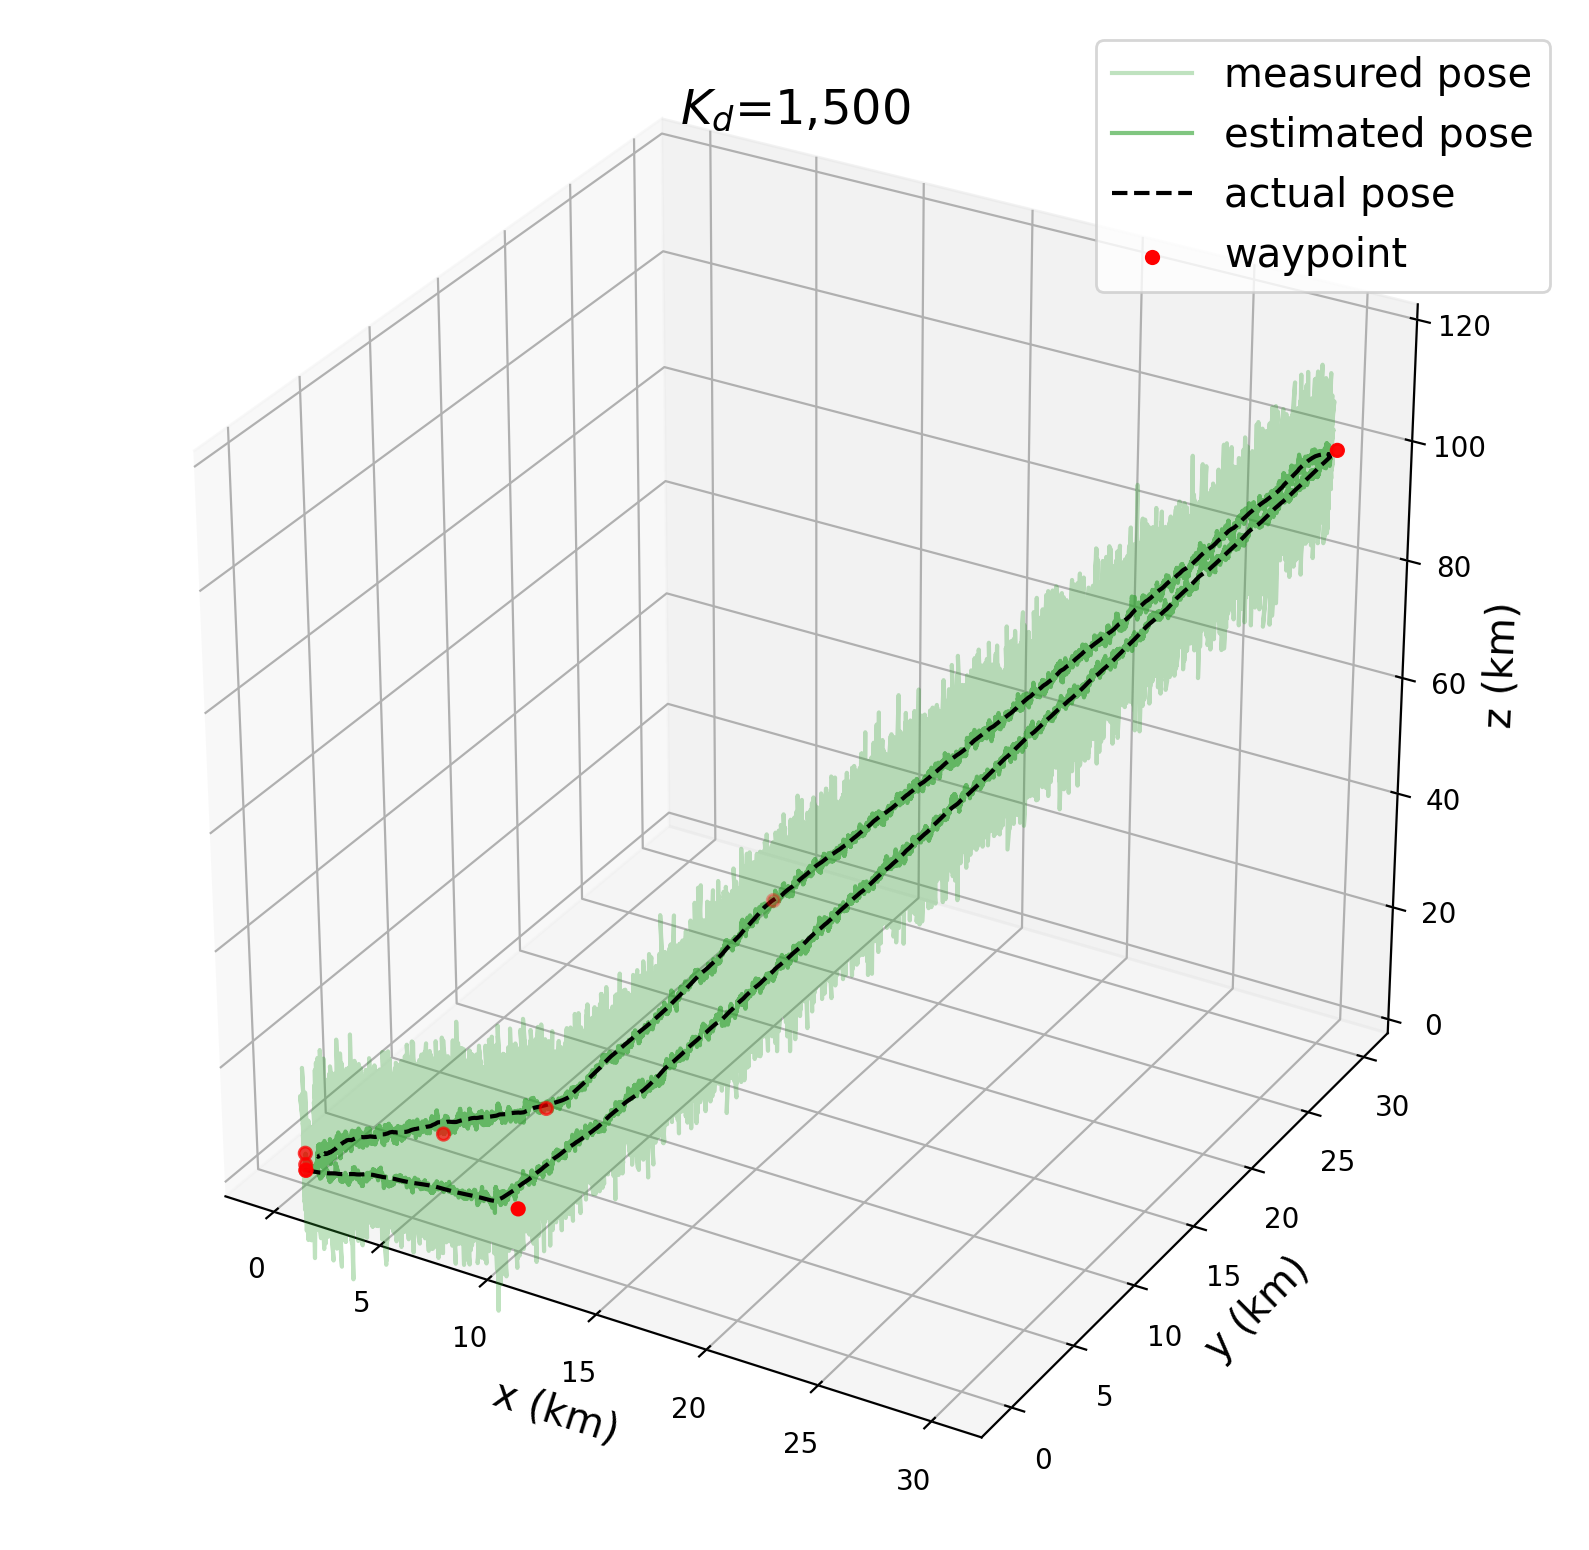
\includegraphics[width=\linewidth]{figures/Dgain_D15_3d.png}
		\caption{$K_d=1,500$}
	\end{subfigure} 
	
	\caption{Two-dimensional plot (left column: a, c, and e) and three-dimensional plot (right column: b, d, and f) of the measured trajectories and the estimated trajectories with $K_d=500$ (blue), $K_d=100$ (orange), and $K_d=1,500$ (green).}
	\label{fig:exp_Dgain}
\end{figure}

 The result of the second experiment is shown in Fig.~\ref{fig:exp_Dgain}. The figure presents that, changing $K_d$ has an observable effect on reducing osculation, but it has minor effect on reducing the root-mean-square error between the trajectory and the expected linear segment between waypoints. In all cases, the root-mean-square-error values are approximately 7.0 km. Using $K_d=500$ gives the error of 7.10 km, while using $K_d=1,500$ gives the error of 6.98 km due to decreased oscillation.

\subsection{Experiment 3: Guidance System}
\label{sec:exp_guidance}

Fixing $\lambda_Q=1$, $:\lambda_R=1,000$, $K_p=1,000$ and $K_d=1,500$, the third experiment compares four sets of guidance parameter $\eta_e$ and $\eta_\Delta$. Those are $\eta_e=0.1\:\&\:\eta_\Delta=150$ (blue), $\eta_e=0.1\:\&\:\eta_\Delta=100$ (orange), $\eta_e=1.0\:\&\:\eta_\Delta=100$ (green), and $\eta_e=2.0\:\&\:\eta_\Delta=100$ (purple).



\begin{figure}[]
	\centering
	\begin{subfigure}[t]{0.24\textwidth}
		\centering
		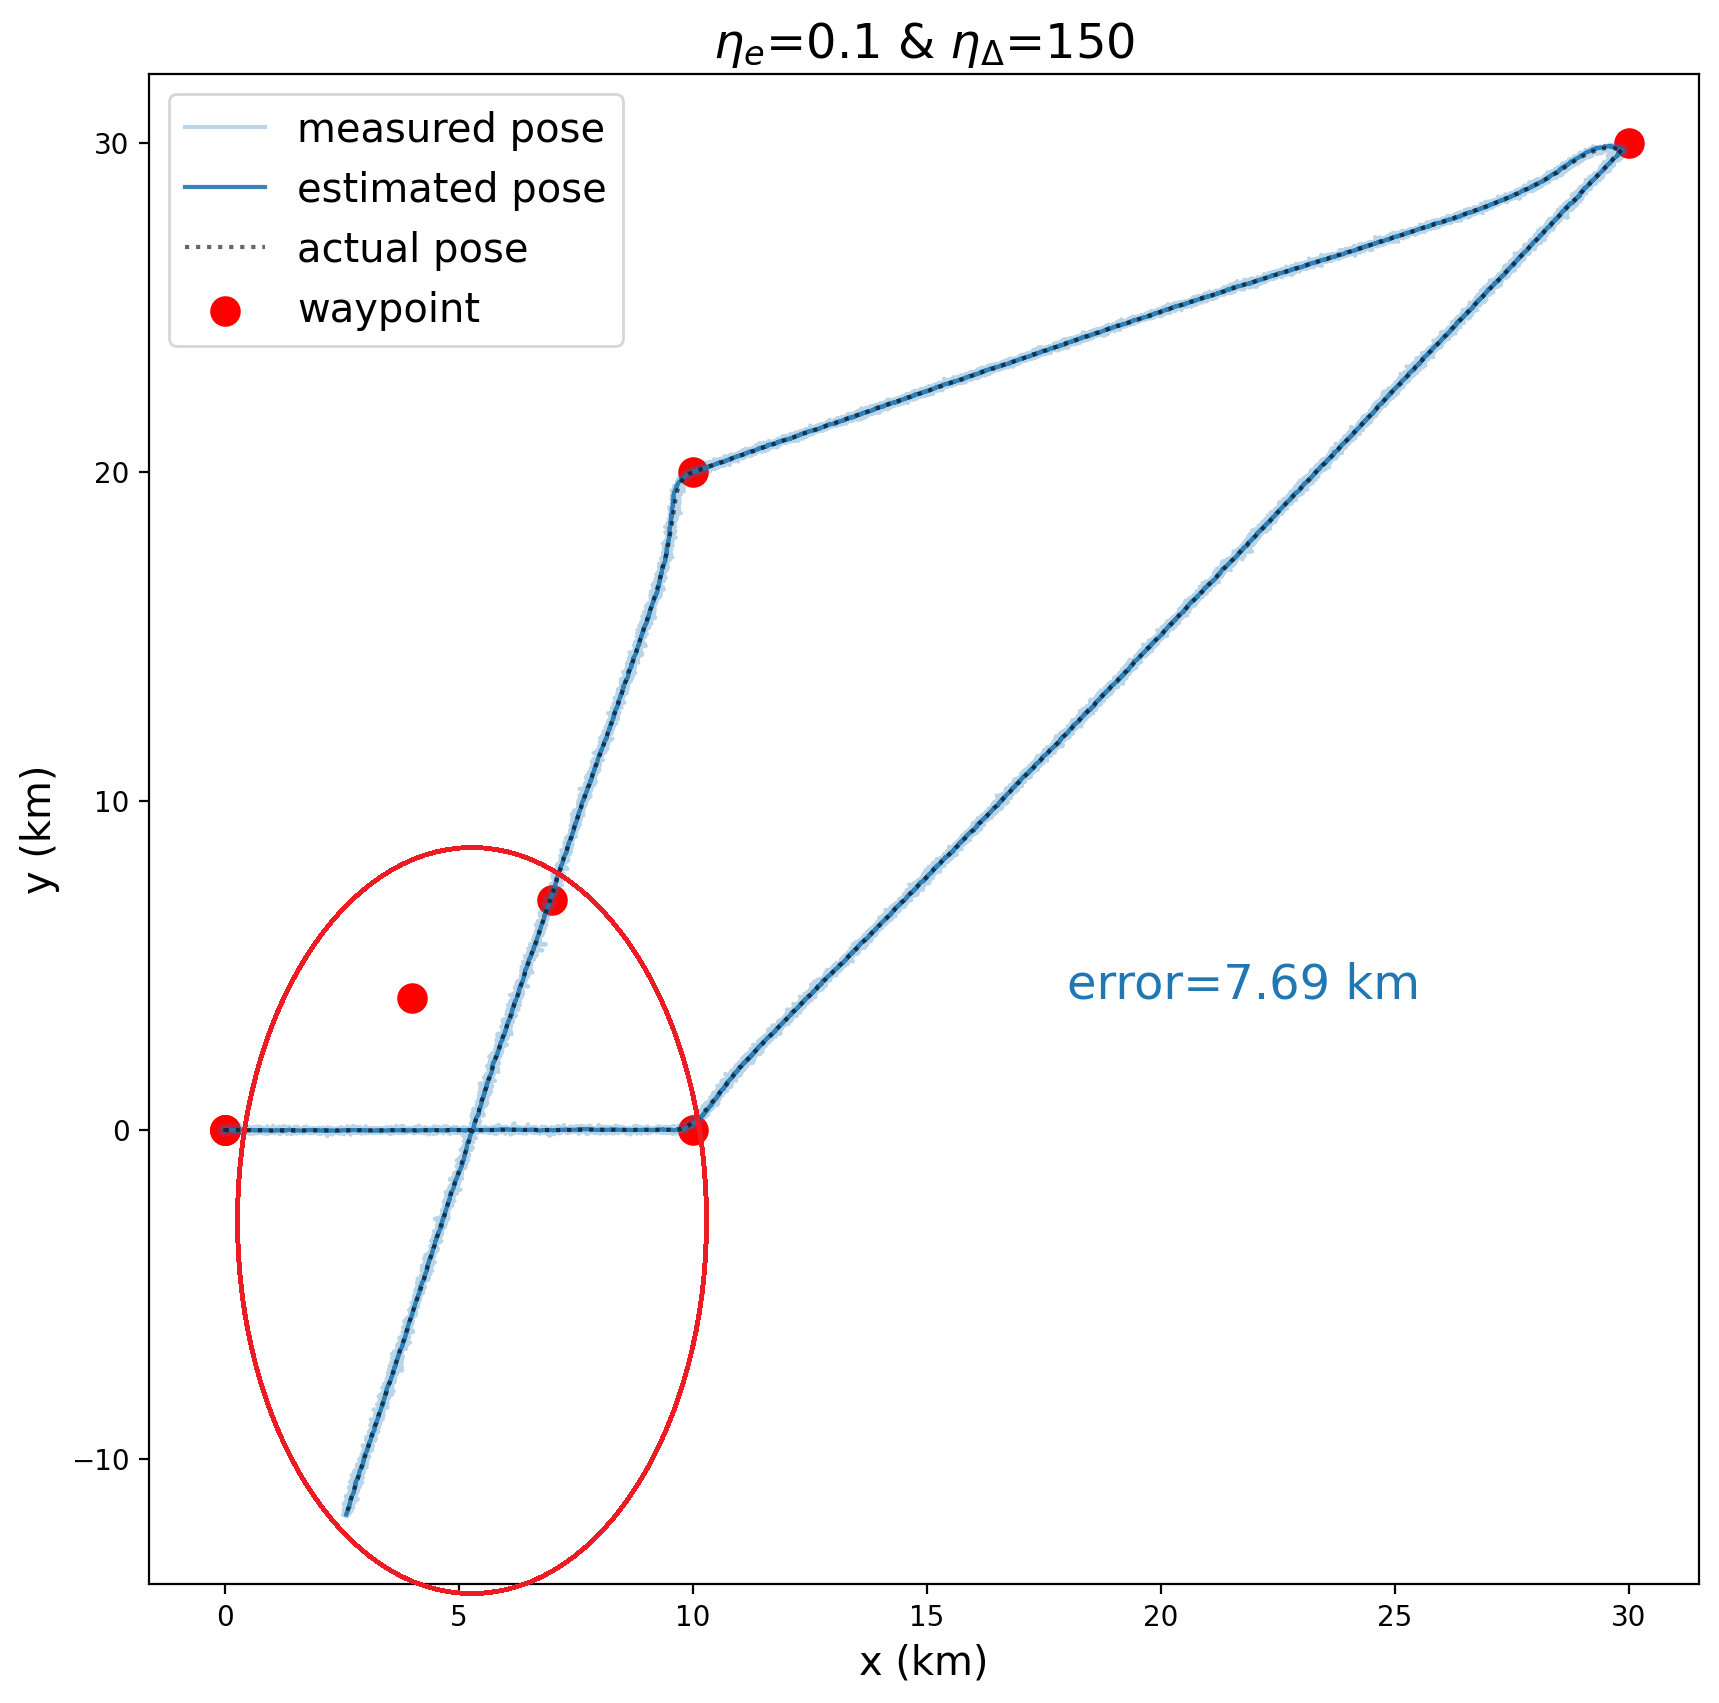
\includegraphics[width=\linewidth]{figures/lookahead_eta_01_150_2d.png}
		\caption{$\eta_e=0.1\:\&\:\eta_\Delta=150$}
	\end{subfigure} 
	\hfill
	\begin{subfigure}[t]{0.24\textwidth}
		\centering
		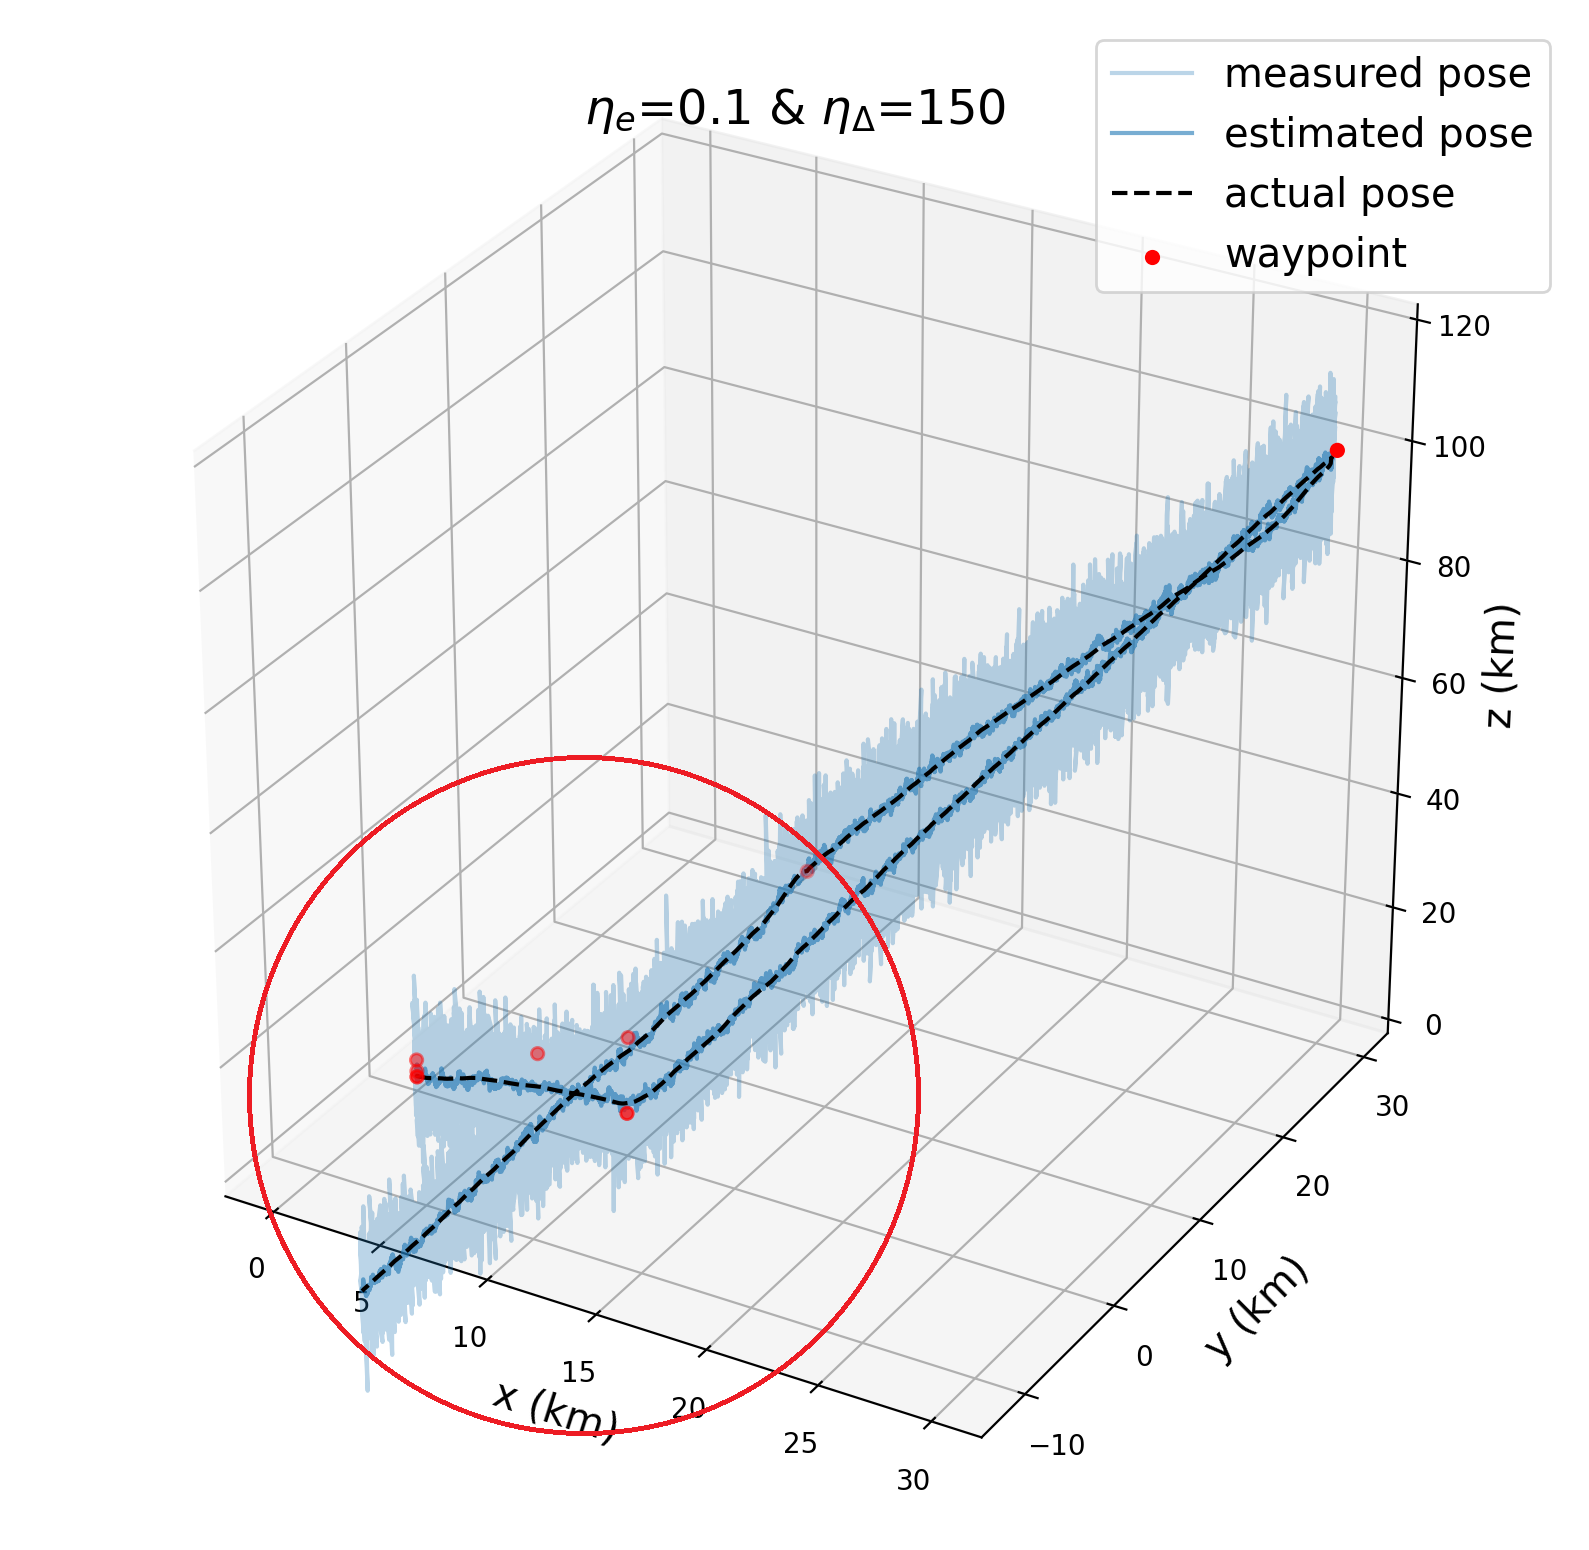
\includegraphics[width=\linewidth]{figures/lookahead_eta_01_150_3d.png}
		\caption{$\eta_e=0.1\:\&\:\eta_\Delta=150$}
	\end{subfigure} \\
	\hfill
	\begin{subfigure}[t]{0.24\textwidth}
		\centering
		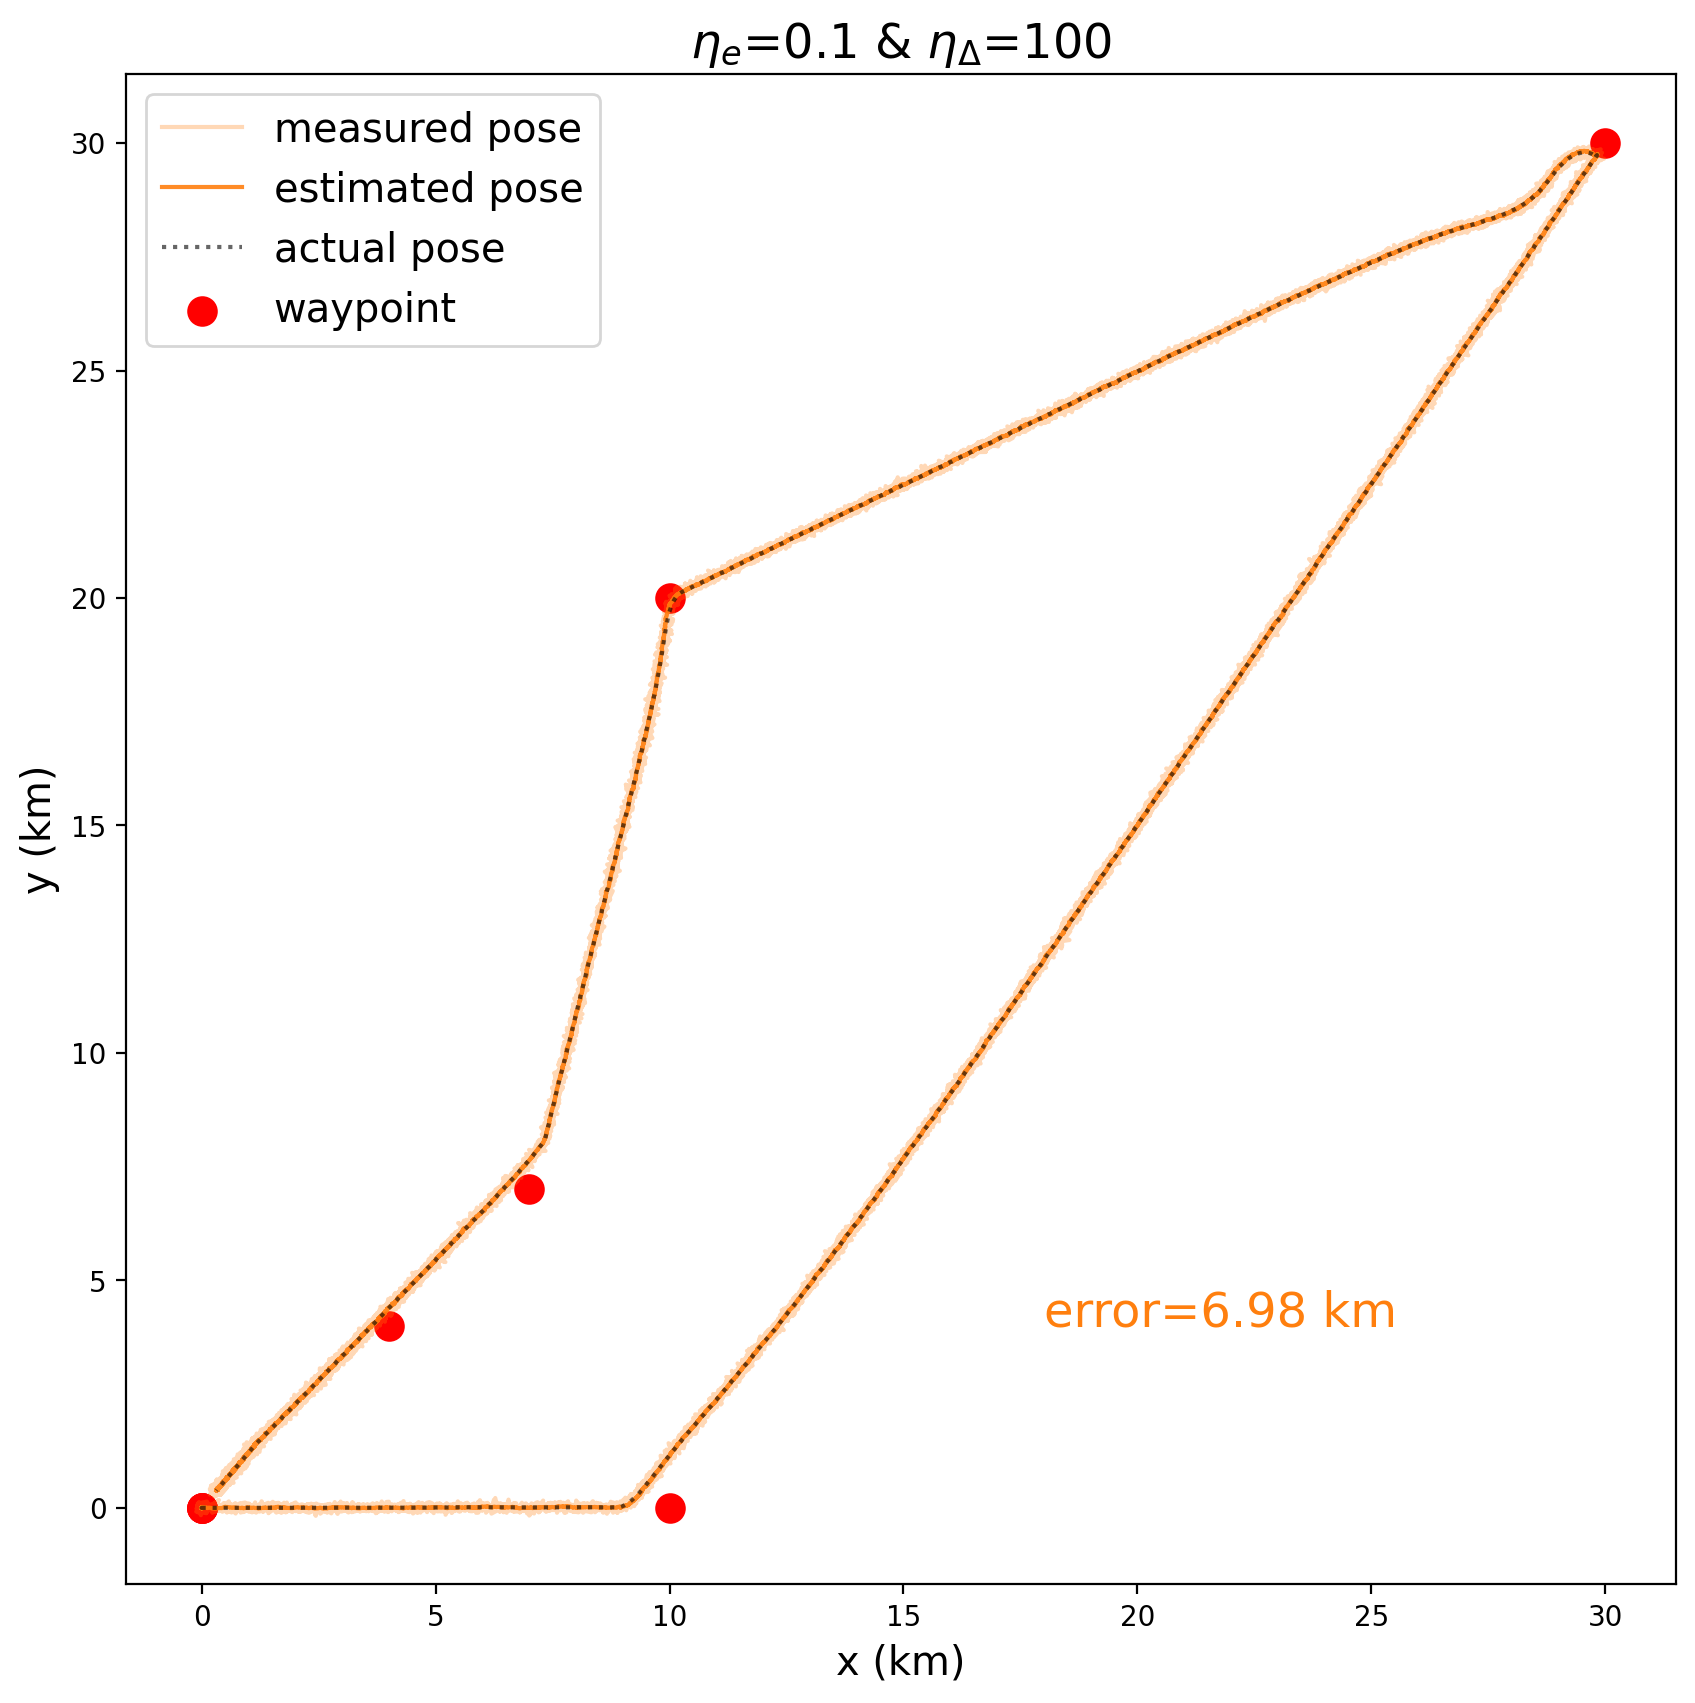
\includegraphics[width=\linewidth]{figures/lookahead_eta_01_100_2d.png}
		\caption{$\eta_e=0.1\:\&\:\eta_\Delta=100$}
	\end{subfigure} 
	\hfill
	\begin{subfigure}[t]{0.24\textwidth}
		\centering
		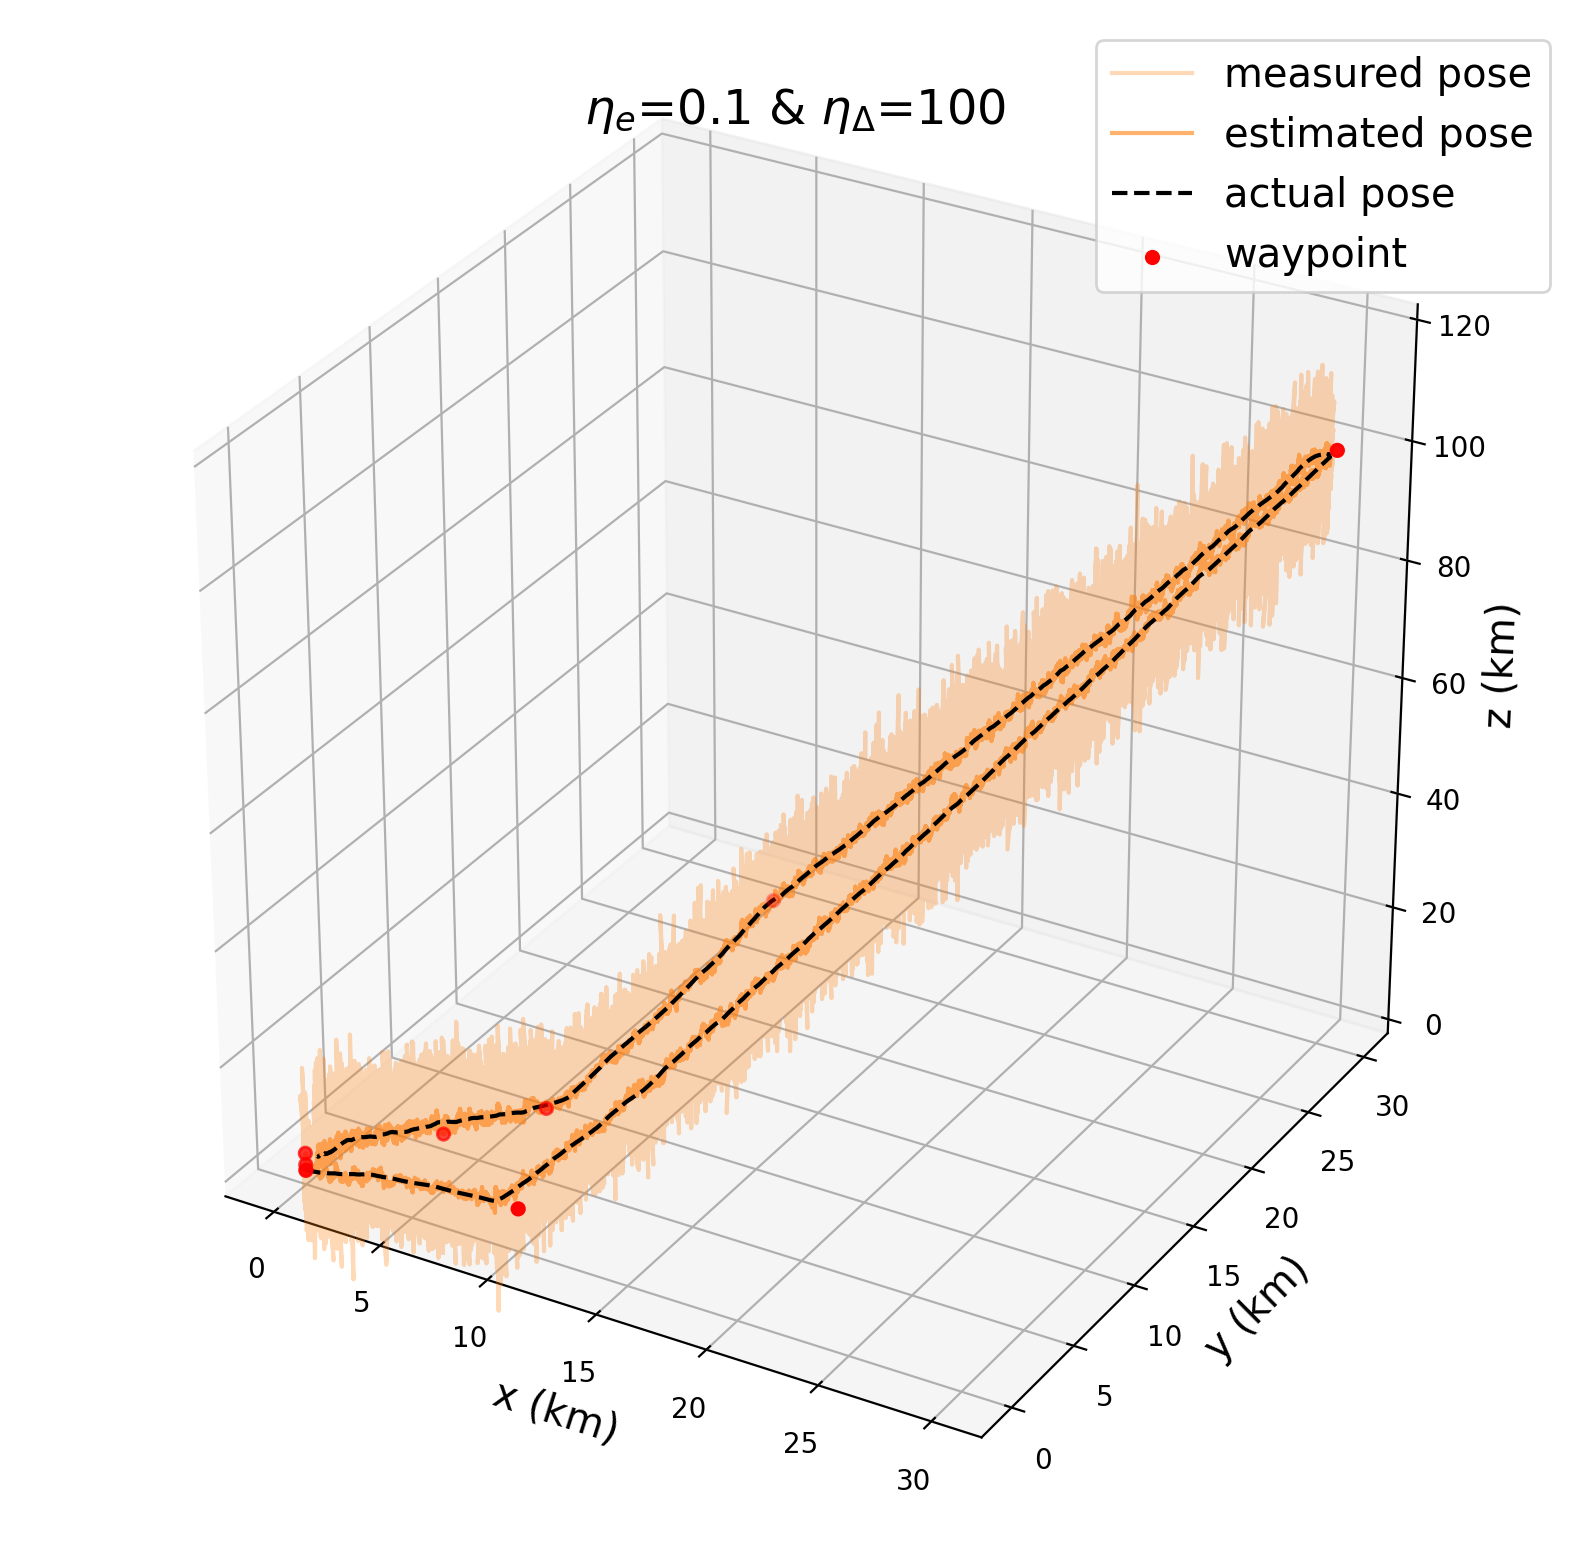
\includegraphics[width=\linewidth]{figures/lookahead_eta_01_100_3d.png}
		\caption{$\eta_e=0.1\:\&\:\eta_\Delta=100$}
	\end{subfigure} \\
	\hfill
	\begin{subfigure}[t]{0.24\textwidth}
		\centering
		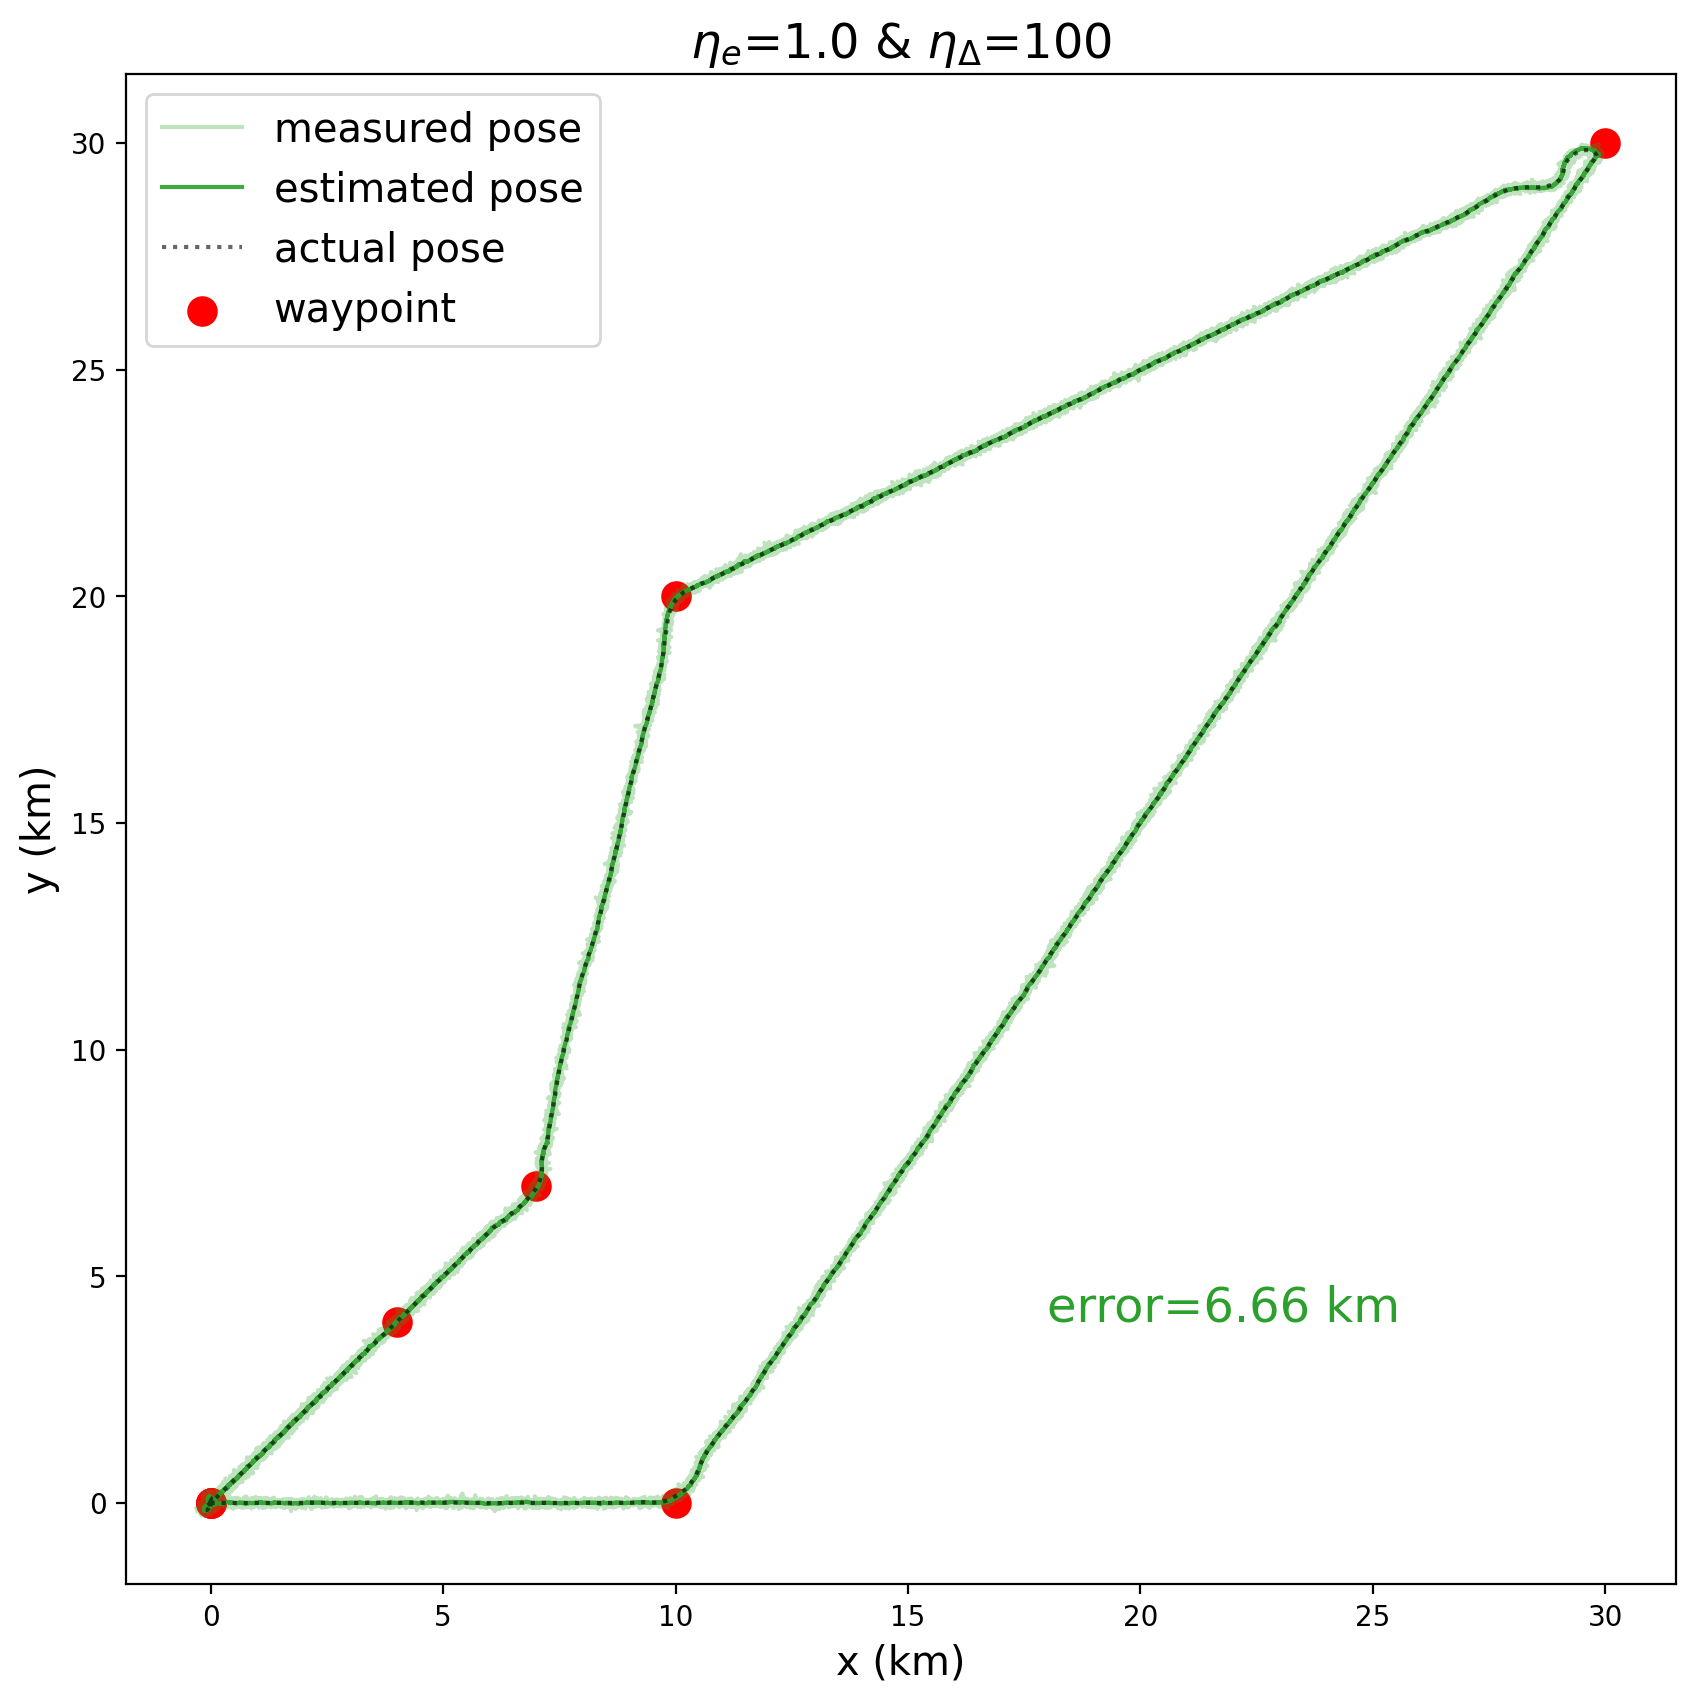
\includegraphics[width=\linewidth]{figures/lookahead_eta_10_100_2d.png}
		\caption{$\eta_e=1.0\:\&\:\eta_\Delta=100$}
	\end{subfigure} 
	\hfill
	\begin{subfigure}[t]{0.24\textwidth}
		\centering
		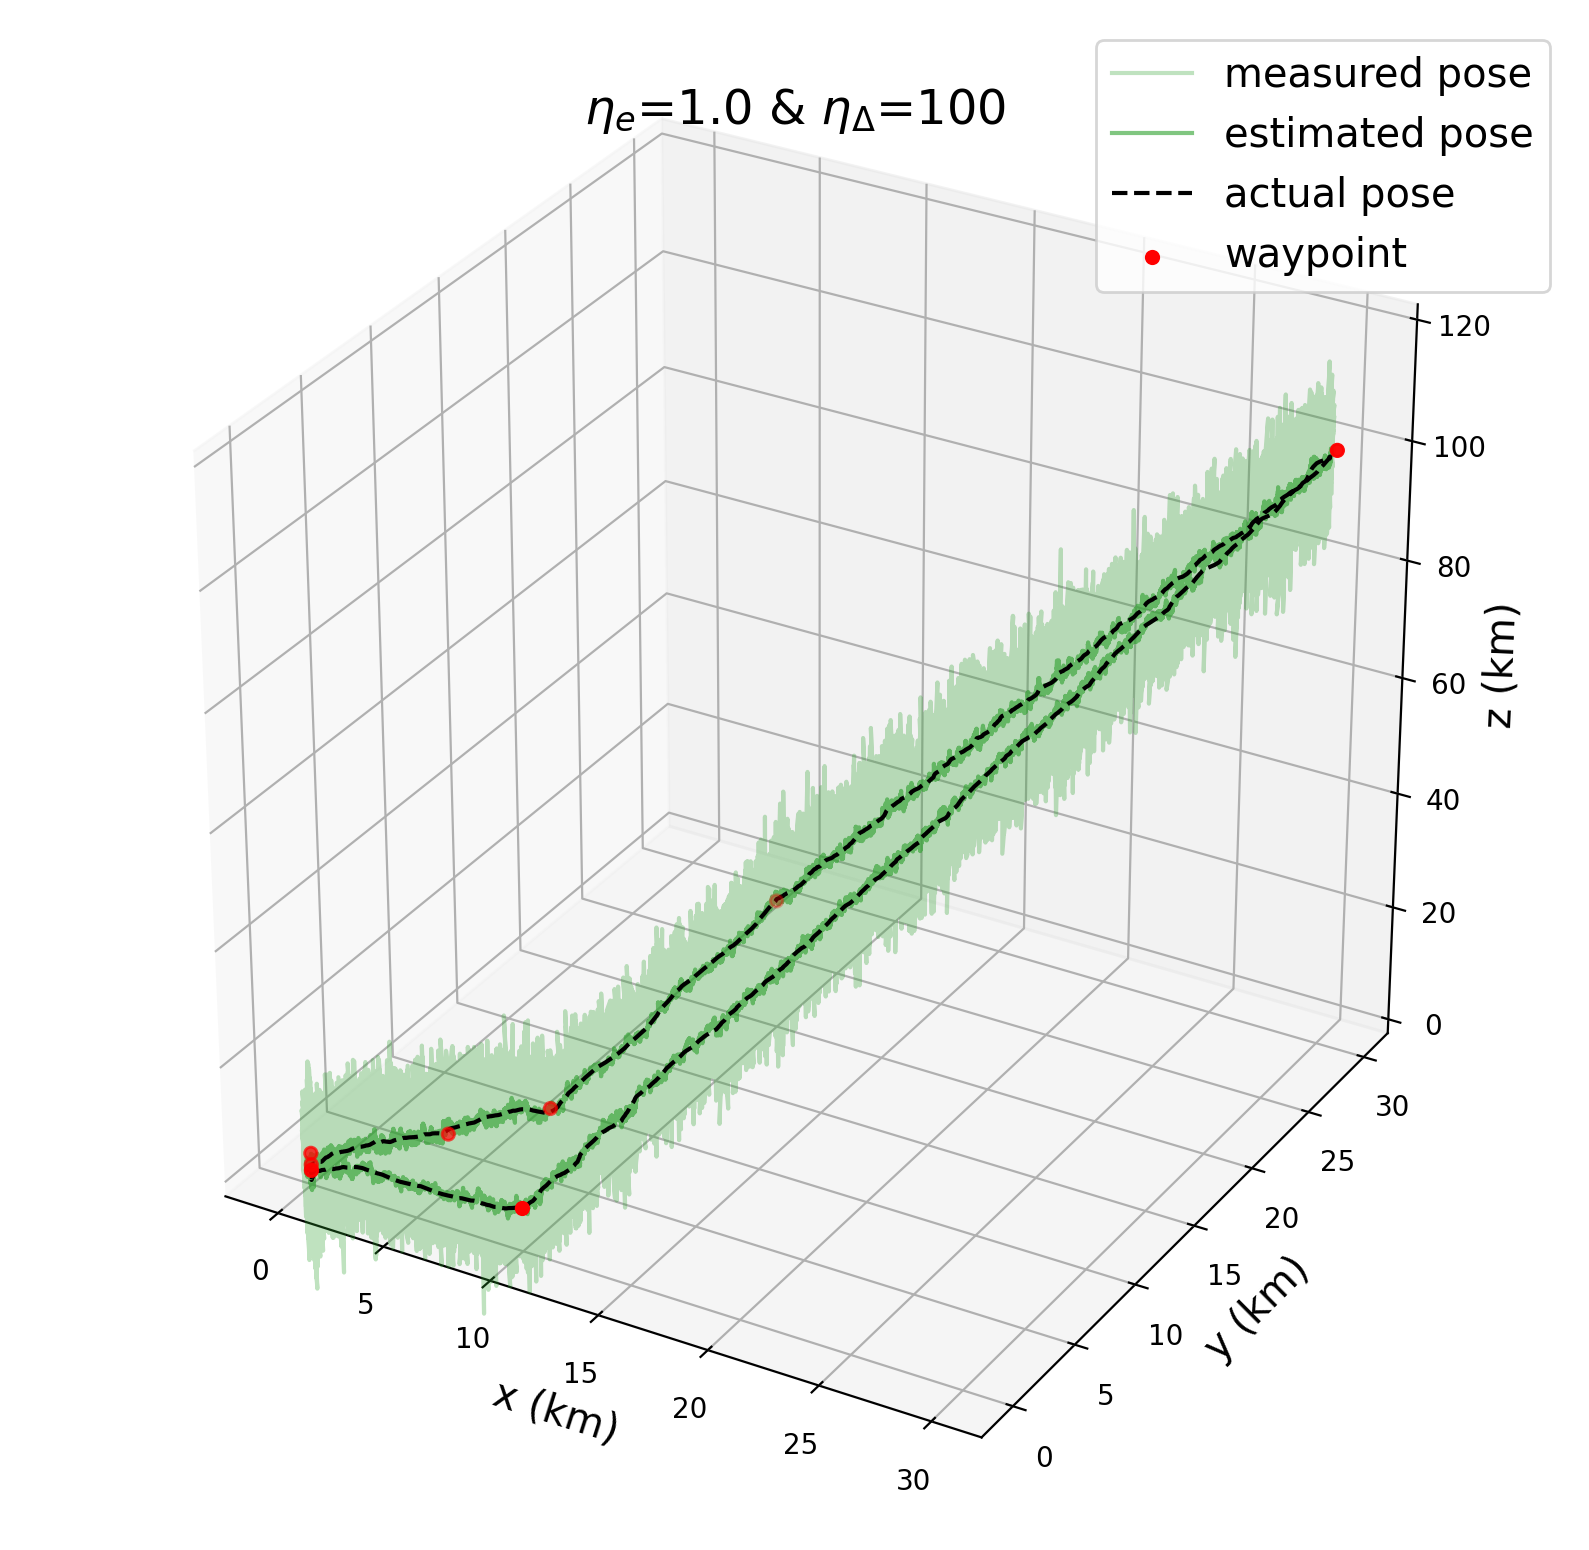
\includegraphics[width=\linewidth]{figures/lookahead_eta_10_100_3d.png}
		\caption{$\eta_e=1.0\:\&\:\eta_\Delta=100$}
	\end{subfigure} \\
	\hfill
	\begin{subfigure}[t]{0.24\textwidth}
		\centering
		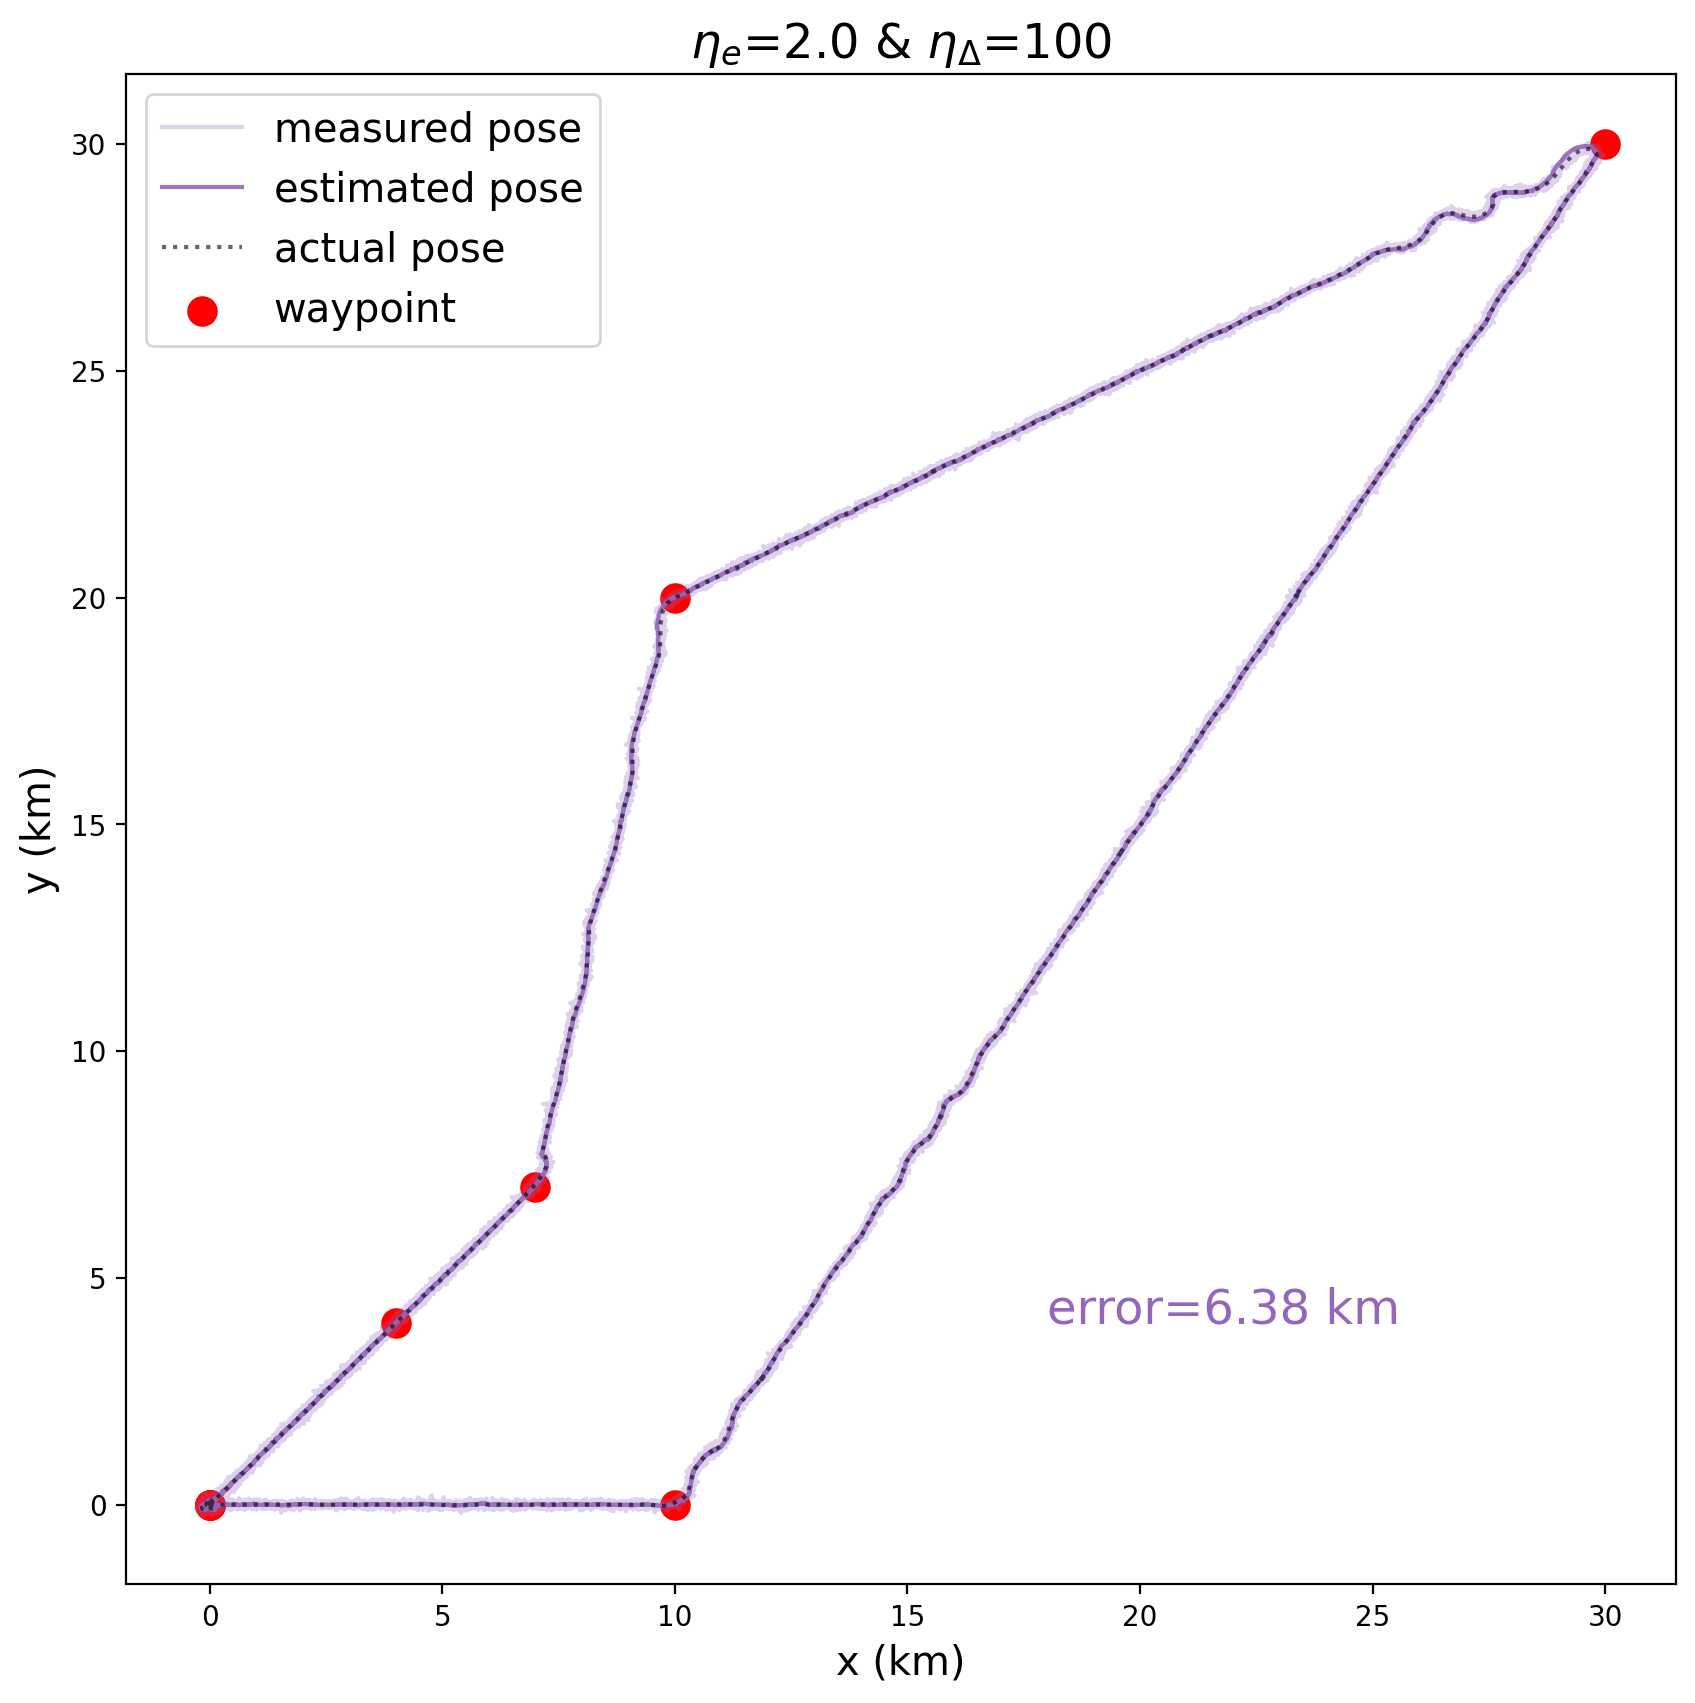
\includegraphics[width=\linewidth]{figures/lookahead_eta_20_100_2d.png}
		\caption{$\eta_e=2.0\:\&\:\eta_\Delta=100$}
	\end{subfigure} 
	\hfill
	\begin{subfigure}[t]{0.24\textwidth}
		\centering
		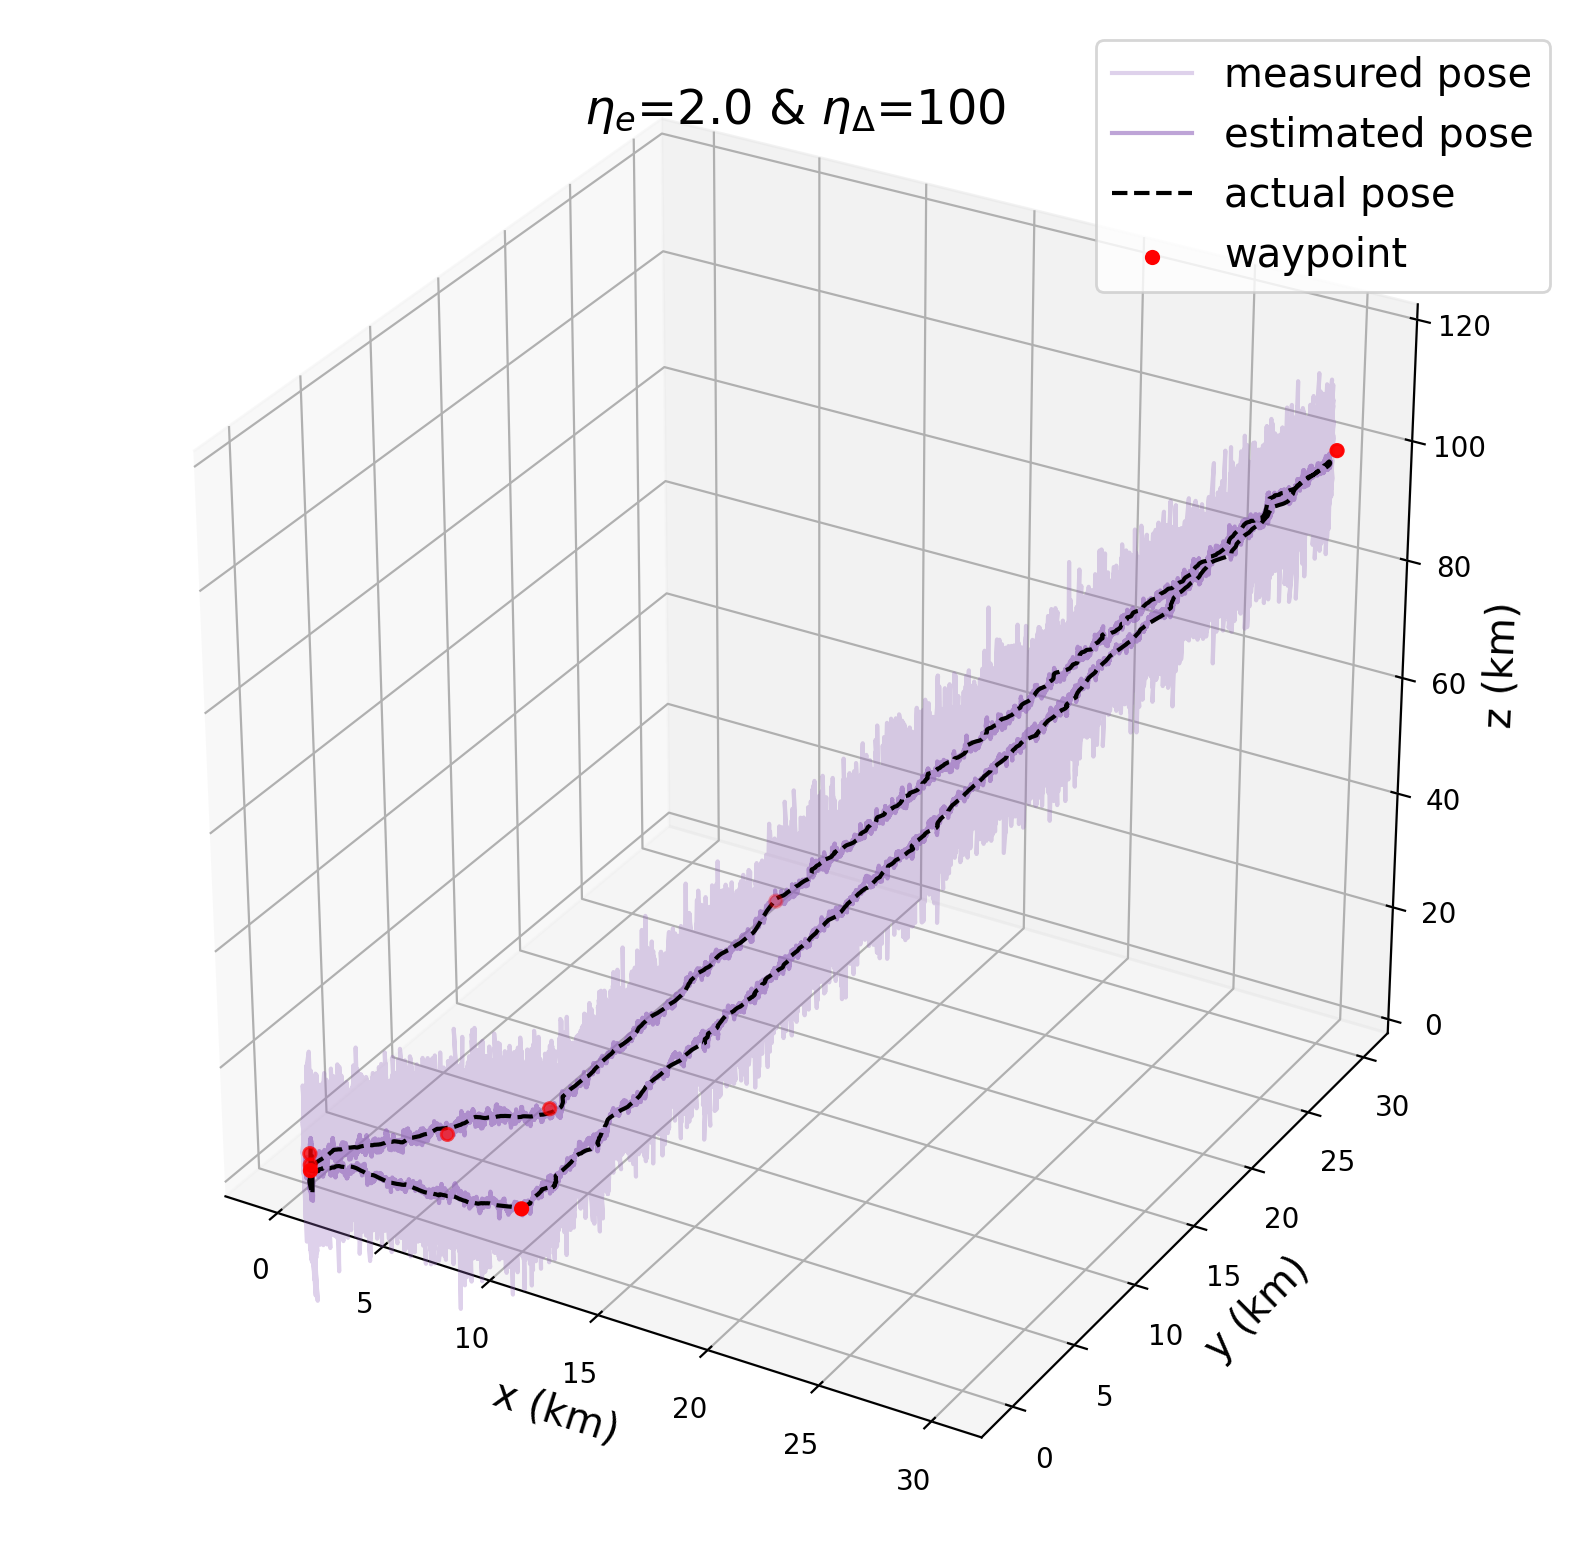
\includegraphics[width=\linewidth]{figures/lookahead_eta_20_100_3d.png}
		\caption{$\eta_e=2.0\:\&\:\eta_\Delta=100$}
	\end{subfigure} 
	
	\caption{Two-dimensional plot (left column: a, c, e, and g) and three-dimensional plot (right column: b, d, f and h) of the measured trajectories and the estimated trajectories with $\eta_e=0.1\:\&\:\eta_\Delta=150$ (blue), $\eta_e=0.1\:\&\:\eta_\Delta=100$ (orange), $\eta_e=1.0\:\&\:\eta_\Delta=100$ (green), and $\eta_e=2.0\:\&\:\eta_\Delta=100$ (purple).}
	\label{fig:exp_lookahead}
\end{figure}

 The result of the third experiment is shown in Fig.~\ref{fig:exp_lookahead}. The figure presents that, changing increasing $\eta_e$ improves the response of the system, while increasing $\eta_\Delta$ disable the spaceship to move between close waypoints. Setting $\eta_\Delta$ to 100 seems to be an optimal point. If we increase it beyond this, the x-wing fighter will lose the ability to reach the next waypoint that locates close to the previous one. The spaceship might be unable to reach the acceptance sphere as highlighted by the red circles in Fig.~\ref{fig:exp_lookahead}(a,b). This is because, the lookahead distance go over the next waypoint, and the x-wing fighter's guidance system cannot see it. $\eta_e$ has a significant effect in reducing the root-mean-square error between the trajectory and the expected linear segment between waypoints. The error drops from 6.98 km to 6.66 km if $\eta_e=1.0$ and to 6.38 km if $\eta_e=2.0$. Setting this value to high can causes multiple oscillation even if the spaceship perfectly stays on a strength path for a while, as shown in Fig.~\ref{fig:exp_lookahead}(g,h). 
 
 The most appropriate set of parameters is found to be $\lambda_Q=1$, $:\lambda_R=1,000$, $K_p=1,000$ $K_d=1,500$, $\eta_e=1.0$, and $\eta_\Delta=100$. With this set of parameters, the autonomous x-wing fighter is simulated, and the video is available at \href{https://youtu.be/vUd8cK0Ot9s}{\url{https://youtu.be/vUd8cK0Ot9s}}.

\begin{figure}[!h]
	\centering
	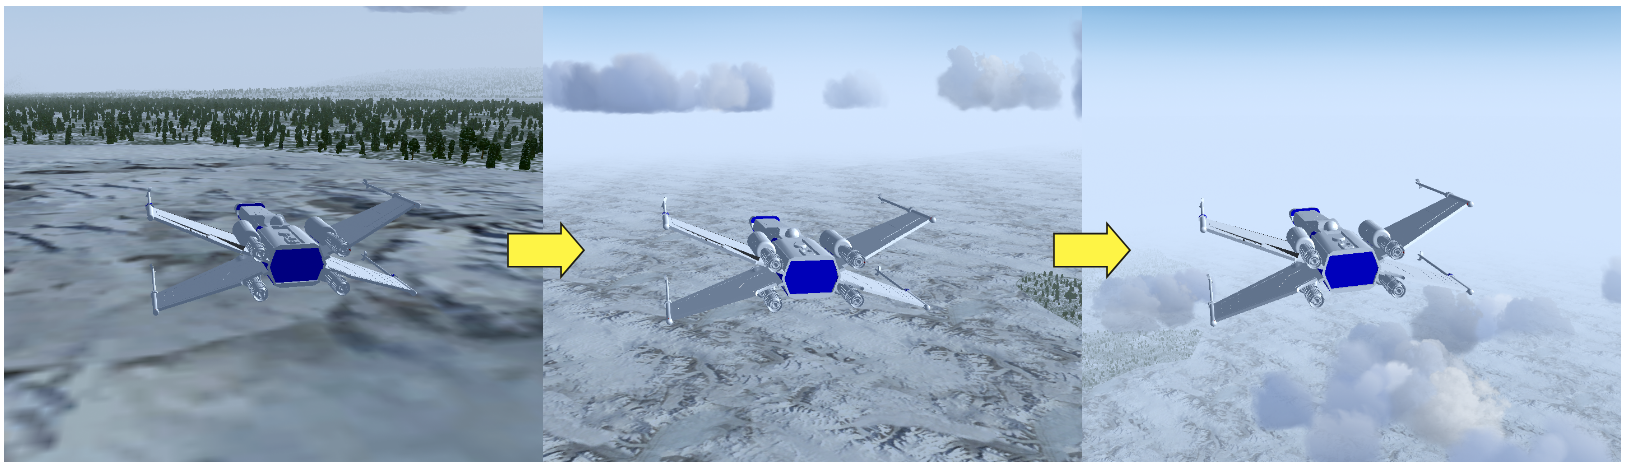
\includegraphics[width=1.0\linewidth]{figures/screenshots}
	\caption{Screenshots from the demonstration video. The video is available at \href{https://youtu.be/vUd8cK0Ot9s}{\url{https://youtu.be/vUd8cK0Ot9s}}.}
	\label{fig:screenshot}
\end{figure}




\section{Discussion and Conclusion}
\label{sec:conclusion}
This project aims to verify if the existing guidance, navigation, and control techniques can achieved a comparable simulation result to the science friction spaceship, star wars' x-wing fighter, introduced nearly 50 years ago. 

The simulation results presented in this report supports that it is possible to control a sci-fi star wars' x-wing fighter using existing guidance, navigation, and control techniques. This work illustrates that lookahead-based line-of-sight guidance system, Kalman state estimation, along with proportion-derivative control can navigate a simulated x-wing fighter in a surveillance mission. Nevertheless, the control parameters have to be selected carefully. Too high value could cause oscillation and reduce the stability of the system, while inappropriate value could make the mission failed (i.e., being unable to reach the waypoint/target).

More advanced techniques could be utilized to improve the performance. For example, a feedforward control like model predictive control \cite{mpc_drone} could be employed to guarantee robust and optimal behavior. Parameter $\eta_e$ and $\eta_\Delta$ could be adapted online according to the distance between waypoints to improve path following and ensure success. Also, if the real-world measurement noise does not satisfy Gaussian distribution assumption, unscented Kalman filter or particle filter could be used as state estimation.



\bibliographystyle{ieeetran}
\bibliography{bibliography}
\end{document}